\documentclass{WileyMSP-template}

\usepackage{amsmath}

\begin{document}


\pagestyle{fancy}
\rhead{\includegraphics[width=2.5cm]{vch-logo.png}}


\title{Influence of illumination spectrum on dissociation kinetic of iron-boron pairs in silicon}

\maketitle



% Author: Please give full first and last names for authors and include * after the name of all corresponding authors

\author{Oleg Olikh*}
\author{Oleksandr Datsenko}
\author{Serhiy Kondratenko}

% Dedication

\dedication{}






% Affiliations: Please provide adacemic titles (Prof. or Dr.) for all authors where applicable, and include an institutional email address for all corresponding authors
\begin{affiliations}
Prof. O. Olikh, Dr. O. Datsenko, Prof. S. Kondratenko\\
Taras Shevchenko National University of Kyiv, 64/13, Volodymyrska Street, 01601, Kyiv, Ukraine\\
Email Address: olegolikh@knu.ua

%A. N. O. Author\\
%Address

\end{affiliations}


% Keywords: Please provide a minimum of three and a maximum of seven keywords, separated by commas

\keywords{silicon, iron-boron pairs, light-induced dissociation, light source impact}



% Abstract should be written in the present tense and impersonal style (i.e., avoid we), and be at most 200 words long
\begin{abstract}

Please insert your abstract here

\end{abstract}

% Text: Please use section headings and subheadings as specified below. For communications, all section headings apart from Experimental Section should be removed
% Please make the first reference to a display item bold: \textbf{Figure 1}
% Do not abbreviate Figure, Equation, etc.; display items are always singular, i.e., Figure 1 and 2.
% Equations are always singular, i.e., Equation 1 and 2, and should be inserted using the {equation} environment, not as graphics
% Please do not use footnotes in the text, additional information can be added to the Reference list.


\section{Introduction}

Defects significantly impact semiconductor properties.
Although minimizing device dimensions to nanometers shifts some focus from extensive to point defects,
physical properties still rely heavily on the presence and distribution of these irregularities.
Hence, many strategies for enhancing semiconductor structures, including radiation and temperature treatments or certain fabrication conditions, strive to decrease the defect concentration or neutralize its effects \cite{Cai2023,Vobecky2021,Frascaroli2021}.
For instance, in the case of photovoltaic devices, we must understand and optimize the carrier properties tied to defects and impurities  \cite{Cai2023}.
Such controlled alteration methods of the defective subsystem have been generalized under the term ``defect engineering'' and are extremely important from a practical standpoint.

Successful defect engineering hinges on an in-depth understanding of defect properties.
Key factors are defect formation energy, transition energy levels, self-compensating effects, nonradiative recombination caused by defects,
and the mechanism of reconstruction and diffusion  \cite{Cai2023}.
Considering the extraordinary diversity of possible intrinsic and impurity defects, complete information on all of them is lacking even for silicon, which is the most studied semiconductor.
Nevertheless, it must be noted that considerable data have been amassed on silicon, and have a solid understanding of some defects \cite{Juhl2018}.

For instance, such defects are iron impurity, a common, detrimental, and often unavoidable contaminant
in photovoltaic silicon \cite{Frascaroli2021,Sun2021}, and iron-boron pair.
Specifically, iron atoms are known to be at the interstitial sites, and Fe$_i^+$ are highly efficient recombination centers \cite{WeberFe}.
In p-type Si at room temperature, iron atoms are almost predominantly bound in complexes with dopants (B, Ga, Al, In).
This defect demonstrates bistable behavior: the stable state is defined by the configuration in which the Fe occupies
the first nearest tetrahedral interstitial site closest to the substituent atom,
whereas, in the metastable configuration, Fe is at the second $T_d$ interstitial site \cite{FeB:PhysRevB49}.
The energy levels associated with iron and its complexes, as well as the respective carriers capture cross-sections, are well-established \cite{Juhl2018,ROUGIEUX2018}.
Among the acceptor-iron pairs, the complex FeB is the most thoroughly investigated,
primarily due to the widespread use of Si:B in the fabrication of various devices, such as solar cells.
However, it is worth mentioning that gallium is gaining increasing attention as an acceptor dopant whose incorporation,
for instance, can help mitigate the light and elevated temperature-induced degradation \cite{Ning2022}.

The dynamics of FeB pairs are also examined.
It's established that FeB pairs can be dissociated through illumination, minority carrier injection, and thermal treatment at 200~$^\circ$C \cite{FeBAssJAP2014}.
In the context of illumination, the dissociation rate $R_d$ is influenced by the overall carrier generation rate $G$ \cite{FeBLight2,FeBAssJAP2014,FeBKin2019,FeMethod2012}:
\begin{equation}
\label{eqRd}
R_d=K\left(\frac{G}{N_\mathrm{FeB}}\right)^2\,,
\end{equation}
where
$N_\mathrm{FeB}$ is the pair concentration,
$K$ is the constant of material.
To achieve almost complete dissociation of the FeB pair, it is necessary for the illumination power to exceed 0.1~W~cm$^{-2}$ \cite{Macdonald2004}.
The dissociation process of FeB pairs by electron capture unfolds in two stages \cite{KIMERLINGFeB,FeBAssJAP2014}:
the initial stage involves the neutralization of Fe and the elimination of the Coulombic attraction between the pair components.
The mechanism of the second stage is contentious; it may involve either the recharge of the iron ion or the recombination-enhanced defect reaction
(REDR) triggered by electron-hole recombination.


It should be noted that despite the extensive data on the properties of iron-related defects in silicon, intensive research persists.
In particular, efforts focus on analyzing the impact of high-intensive  illumination \cite{FeBStrongIll}
or dopant compensation \cite{Zhu2015},
alongside clarifying the second-stage mechanism of dissociation \cite{Sun2021}
or reassessing recombination parameters \cite{Le2024}.

This study aims to investigate the effect of the light spectrum on the dissociation kinetics of FeB pairs in silicon.
While pair dissociation is typically carried out using a halogen lamp \cite{FeBLight2,Sun2021}
or 904 nm laser \cite{FeBStrongIll,FeBAssJAP2014,lauer2016}, there is limited understanding of how the light source influences this process.
By studying the impact of different illumination spectra on FeB dissociation,
we aim to provide valuable insights for defect engineering and the efficient transformation of detrimental impurity iron atoms into a highly mobile interstitial state
within the active region of a silicon device.
Besides, such information, in our opinion, can help make the right choice between existing options for the second stage of pair decay.




Figure~\ref{fig1} illustrates the main stages of the research. Initially, the dissociation rate of FeB pairs under illumination of the solar cell with different integrated intensities was determined. For this purpose, the dependence of the quantity of interstitial iron atoms formed over time under intense illumination was measured. The concentrations of formed pairs were measured by investigating the kinetics of short-circuit current. Three light sources from different manufacturers were used (further details are described in Section 1).
To determine the carrier generation rate, spectra of sample illumination using various light sources were measured, taking into account the effects of light reflection, absorption by free carriers, and effective absorption depths. The obtained results led to the conclusion that the efficiency of light-induced dissociation increases with decreasing photon wavelength.

\begin{figure}
\centering
  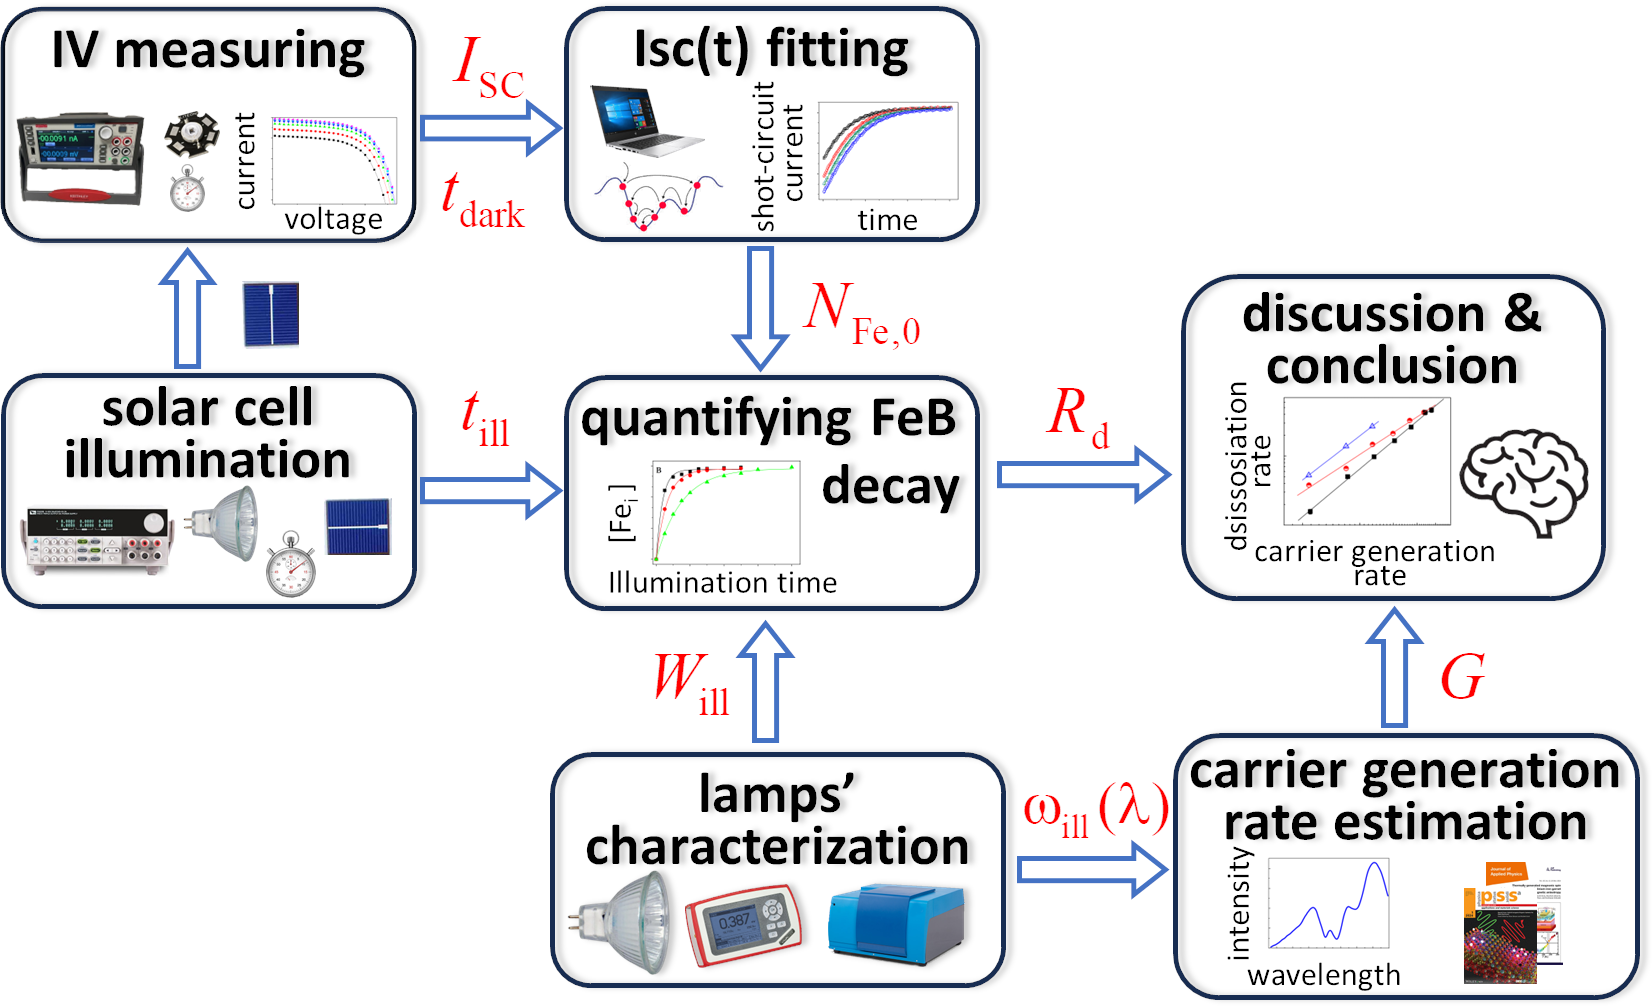
\includegraphics[width=0.5\linewidth]{Fig1.png}
  \caption{Investigation framework}
  \label{fig1}
\end{figure}

In Figure 1, the main stages of the research are illustrated.
First step was determination of the dissociation rate of FeB pairs under illumination with different integrated intensities.
Three light sources from different manufacturers were used (further details are described in Section~\ref{SecExp}).
To measure number of interstitial iron atoms formed over fixed time under strong illumination the kinetics of short-circuit current was used.
The result is presented in Section~\ref{SecR}.
Section~\ref{SecG} deals with estimating the carrier generation rate using spectra of sample illumination and considering the effects of light reflection, absorption by free carriers, and effective absorption depths.
The obtained results showed that the efficiency of light-induced dissociation increases with decreasing photon wavelength --- see Section~\ref{SecLast}.
Finally, we conclude this paper in Section~\ref{SecConsl}.



%\subsection{First Subsection}
%
%
%\subsubsection{First Sub Subsection}
%
%
%\threesubsection{First lowest-level subsection}


\section{Results and Discussion}

\subsection{Dissociation rate determination}\label{SecR}

The equilibrium between free Fe$_i$ and Fe$_i$B$_s$ is known to be determined by the following equations \cite{FeB:kinetic,Sun2021,FeBAssJAP2014}
\begin{equation}
\label{eqReac}
\mathrm{Fe}_i+\mathrm{B}_s  \overset{R_a}{\underset{R_d}{\rightleftharpoons{}}} \mathrm{FeB}\,,
\end{equation}
where
$R_a$ is the association rate.
As a result, the concentration of interstitial iron atoms $N_\mathrm{Fe_i}$ depending on illumination time $t_\mathrm{ill}$ 
during light-induced dissociation can be described as follows \cite{FeBLight2,FeBKin2019,Olikh2021JAP}
\begin{equation}
\label{eqNfeill}
N_\mathrm{Fe_i}(t_\mathrm{ill})=\left(N_\mathrm{Fe,eq}-N_\mathrm{Fe,tot}
\frac{R_d}{R_d+R_a}\right)\exp[-(R_d+R_a)t_\mathrm{ill}]+N_\mathrm{Fe,tot}\frac{R_d}{R_d+R_a}\,,
\end{equation}
where
$N_\mathrm{Fe,tot}$ is the total concentration of the impurity iron,
$N_\mathrm{Fe,eq}$ represents the concentration of unpaired interstitial iron atoms in the equilibrium state 
(in darkness, $N_\mathrm{Fe,eq}=N_\mathrm{Fe_i}(t_\mathrm{ill}=0)$).
It's important to highlight that $N_\mathrm{Fe,eq}$ is significantly influenced 
by temperature and the Fermi level location \cite{FeB:kinetic}. 
Specifically, in the case of p-type Si with a hole concentration of $1.36\times10^{15}$~cm$^{-3}$ 
(which corresponds to the base of the structure under investigation),  
at a temperature of $T=300$~K, $N_\mathrm{Fe,eq}$ constitutes merely about 1\% of $N_\mathrm{Fe,tot}$, 
rendering it negligible for practical considerations. 
However, when the temperature rises to 340~K, the proportion of $N_\mathrm{Fe,eq}$ increases to approximately 14.5\%.

After the cessation of illumination, only the process of association occurs, 
and the time dependence of Fe$_i$ concentration can be expressed as follows \cite{FeB:kinetic,MurphyJAP2011}:
\begin{equation}
\label{eqNFet}
N_\mathrm{Fe_i}(t_\mathrm{dark})=(N_\mathrm{Fe,0}-N_\mathrm{Fe,eq})\times
\exp(-R_a t_\mathrm{dark})+N_\mathrm{Fe,eq}\,,
\end{equation}
where $t_\mathrm{dark}$ is the time after strong illumination stopping,
$N_\mathrm{Fe,0}$ is the concentration of interstitial iron atoms formed after illumination,
$N_\mathrm{Fe,0}=N_\mathrm{Fe_i}(t_\mathrm{dark}=0)=N_\mathrm{Fe_i}(t_\mathrm{ill})$.

The study examined the dependence of $N_\mathrm{Fe,0}$ in silicon solar cells on illumination time $t_\mathrm{ill}$
using different illumination intensities $W_\mathrm{ill}$ ($200-750$~mW) and light sources
(three halogen lamps, labeled as Orion, Osram, and GE, and described in detail in Section~\ref{SecExp}). 
The experiments were conducted at a temperature of 340~K. 
The values of $N_\mathrm{Fe,0}$ were  determined using a methodology \cite{Olikh2022:JMatSci,Olikh2021JAP}
based on the study of the kinetics of short-circuit current $I_{SC}$ under low-intensity monochromatic illumination. 
Specifically, after strong illumination with a duration of $t_\mathrm{ill}$, 
the current-voltage characteristic (IV) of the solar cell was measured every 21 seconds over a time $t_\mathrm{dark}$ interval of approximately 3000 seconds.

Figure~\ref{fig2}a shows some typical IV curves.
It can be seen that upon cessation of illumination, there exists a gradual augmentation in both the short-circuit current and the open-circuit voltage.
This phenomenon is indicative of a decrease in the recombination activity of the defective subsystem, 
which is a result of the transition of interstitial iron to a bound state with an acceptor.
Moreover, at the end of the measurement interval, the minute changes in the IV curves denote that the selected interval of 50 minutes is sufficient to complete the association. 


\begin{figure}
\centering
  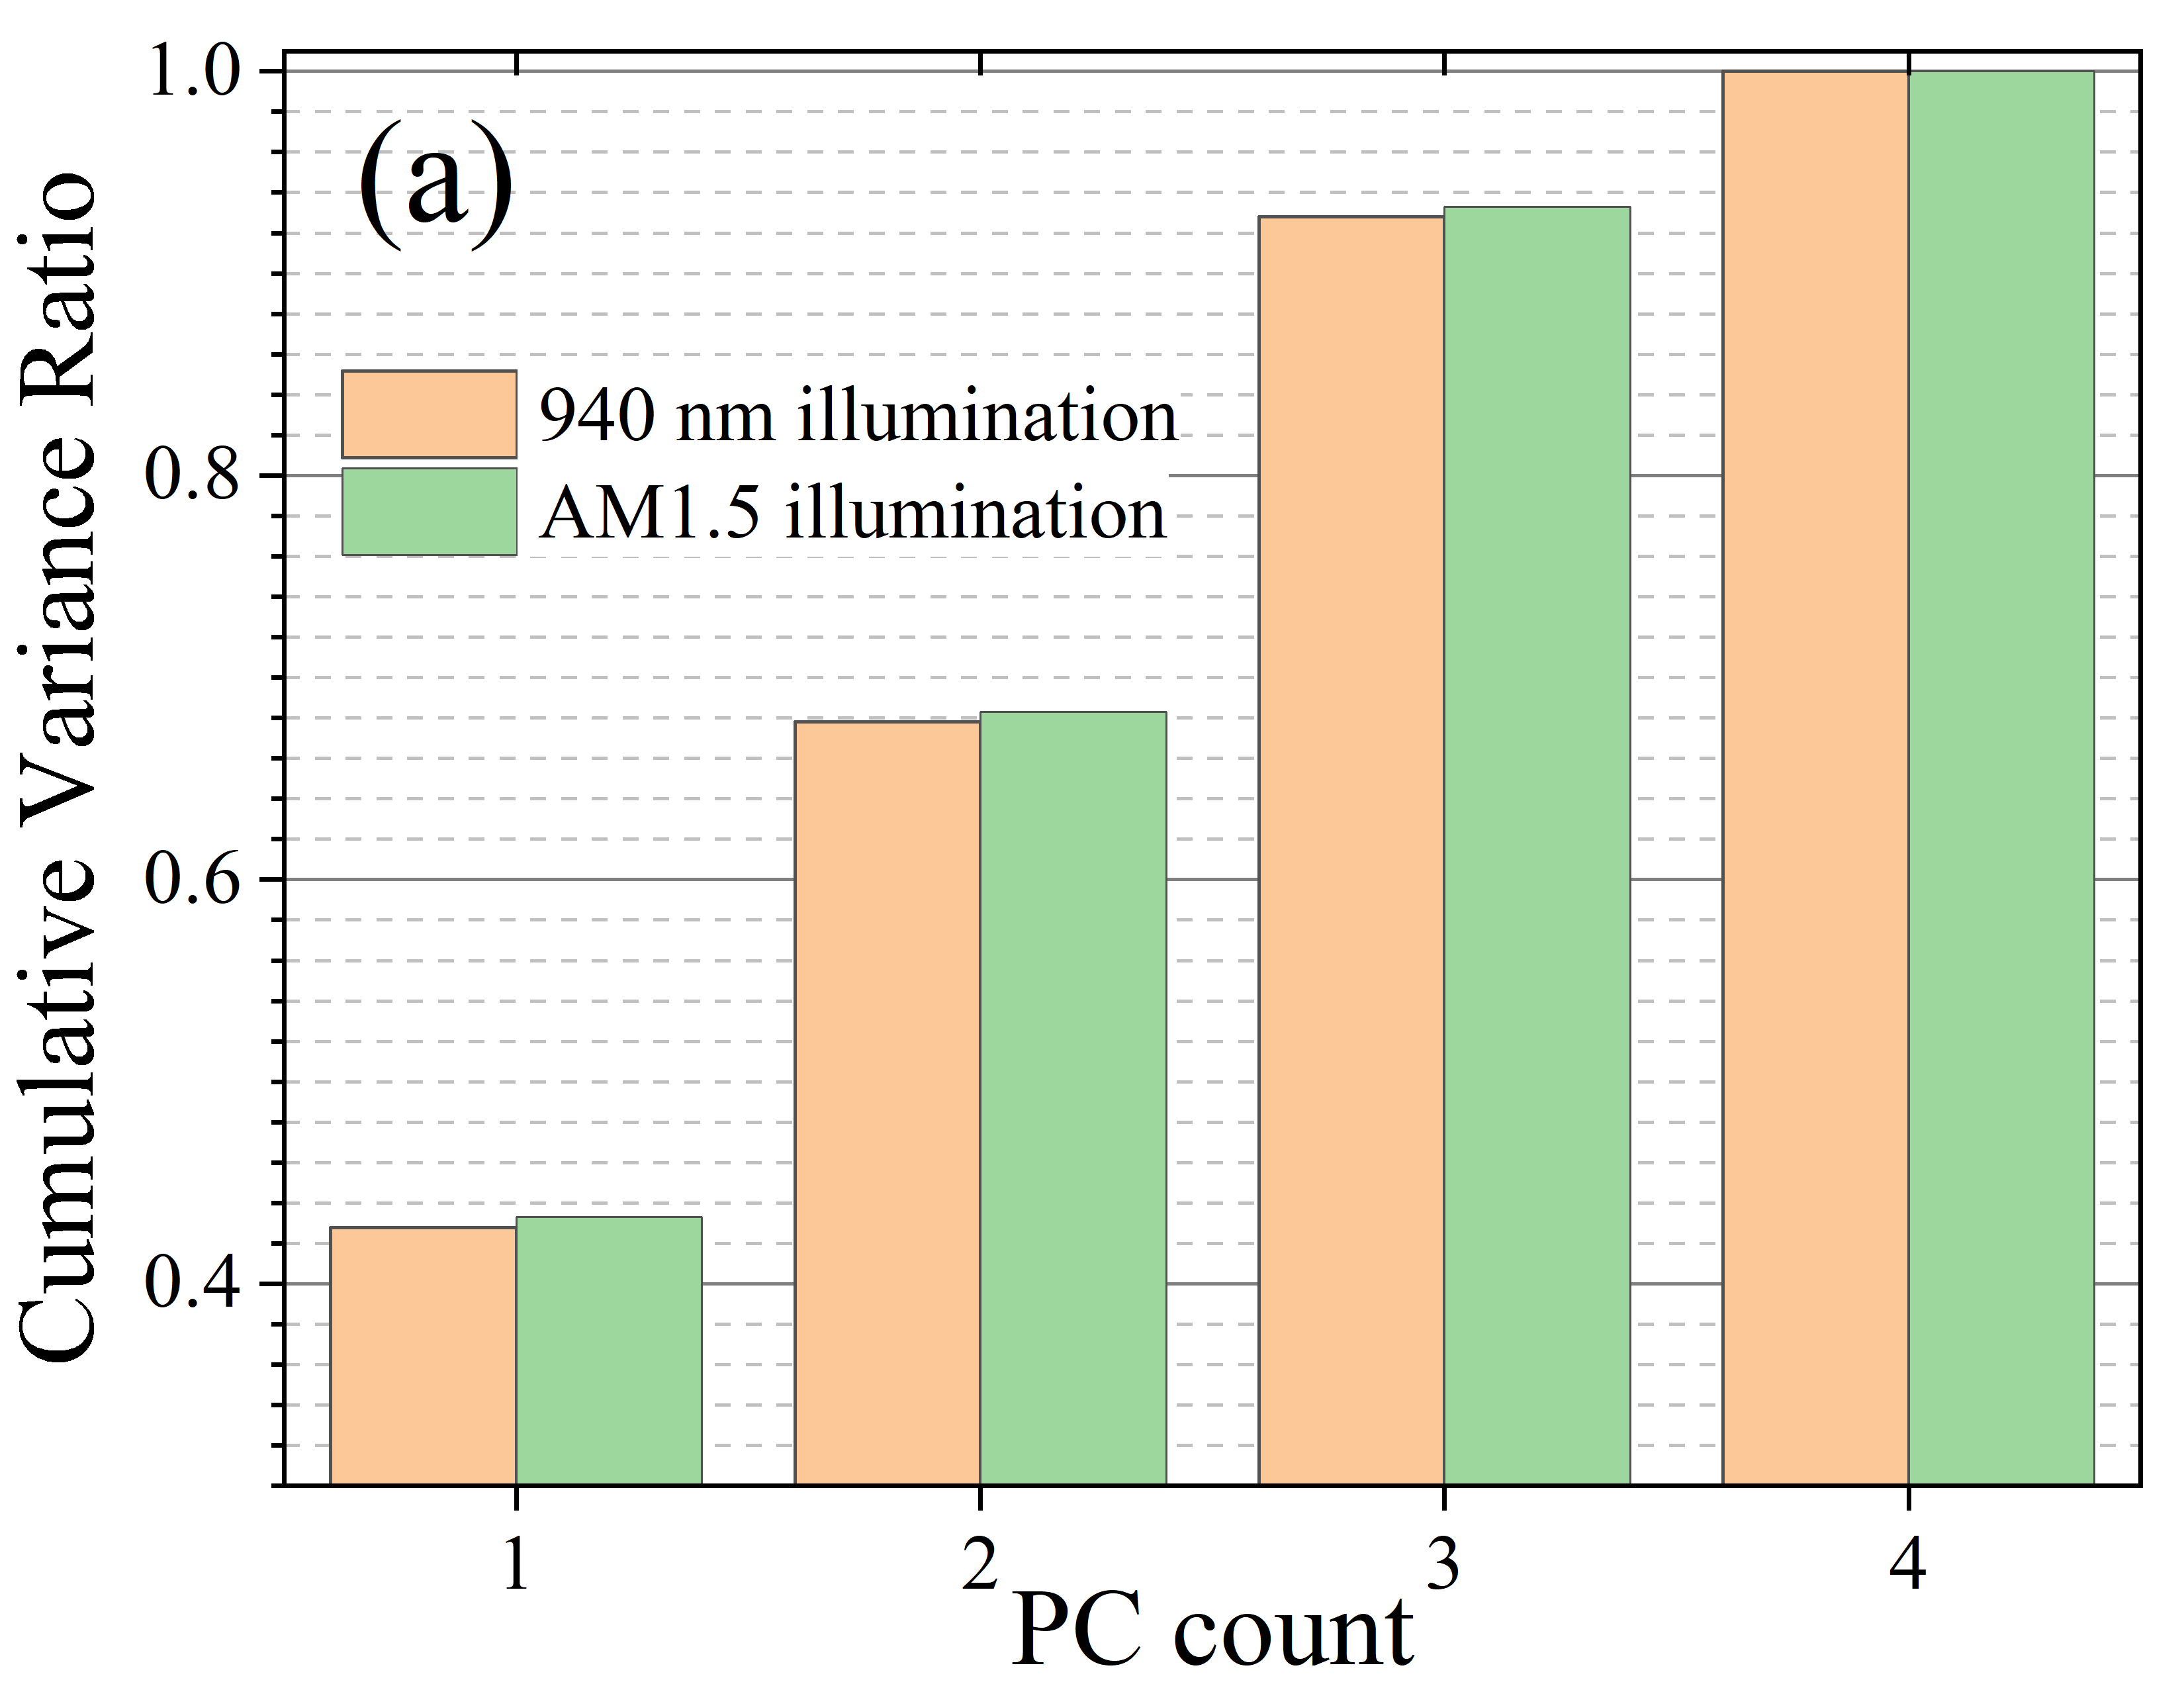
\includegraphics[width=0.4\linewidth]{Fig2a.png}
  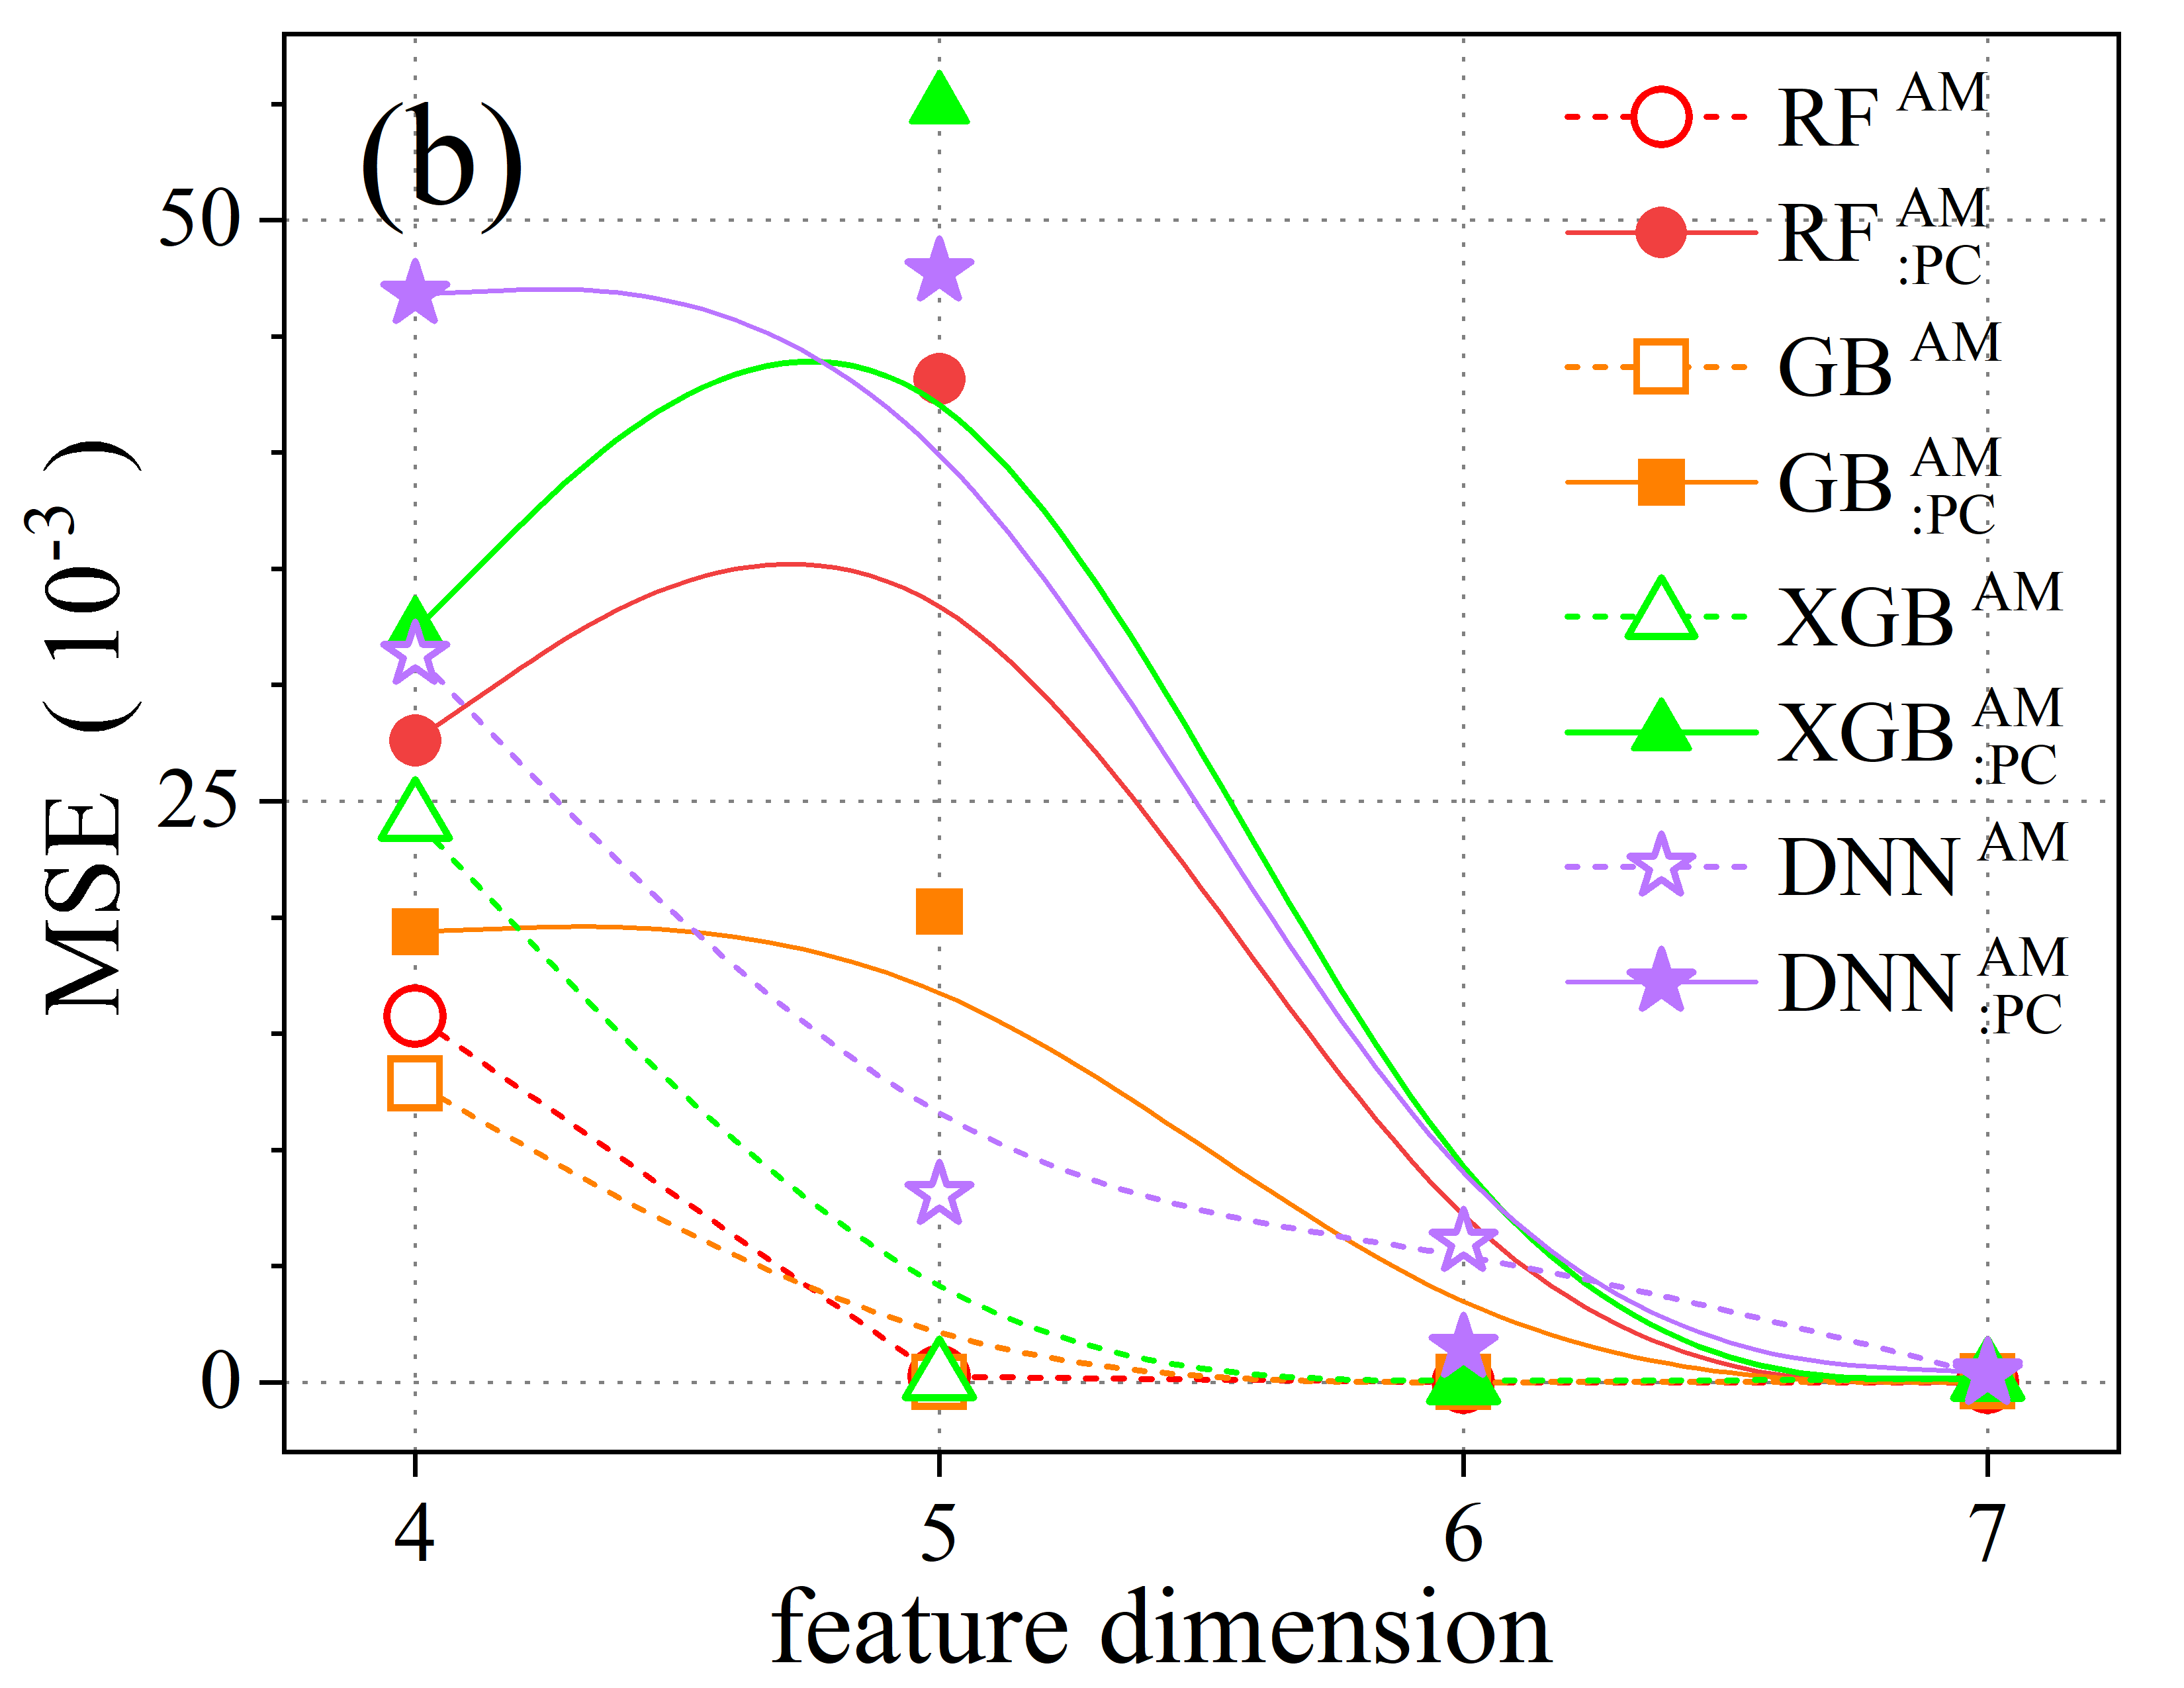
\includegraphics[width=0.4\linewidth]{Fig2b.png}
  \caption{Typical current-voltage characteristics measured
  under low-intensive (LED) illumination across different periods following exposure to strong light (halogen lamp) (panel a) and
  short circuit current plotted as a function of the time after high-intensive illumination (panel b).
  %The marks are the experimental results and the lines are given for convenience only (b) and the curves fitted according to \cite{Olikh2022:JMatSci,Olikh2021JAP}.
  The marks are the experimental results and the lines on panel b are the curves fitted according to \cite{Olikh2022:JMatSci,Olikh2021JAP}.
  Light sources: GE (a), Osram (b).
  $t_\mathrm{ill}$, s: 50 (a), 5(b).
  $W_\mathrm{ill}=400$~mW (a).
  $T=340$~K.}
  \label{fig2}
\end{figure}

Figure~\ref{fig2}b illustrates the dependencies $I_{SC}(t_\mathrm{dark})$ after illumination with different intensities. 
As previously shown \cite{Olikh2021JAP}, the magnitude of the change in $I_{SC}$ after the dark recovery period 
inherently correlates with the concentration of Fe$_i$ formed as a result of light-induced dissociation of FeB pairs. 
From examining the presented data, it is evident that escalating $W_\mathrm{ill}$ leads to an augmentation in the dissociation efficiency. 
Concurrently, the recovery time remains insensitive to the illumination parameters, which conforms to expectations, 
given that the latter is determined by $R_a$ --- see Equation~(\ref{eqNFet}).

Зазначимо, що окрім $N_\mathrm{Fe,0}$ values, використана методика дозволяє оцінити the energy of Fei migration Em and

τSRH,others is the bulk SRH lifetime which stems from defects other than FeGa

τother describes further
recombination channels (other impurities, lattice defects, surface
recombination).

Shockley–Read–Hall (SRH)

\begin{figure}
\centering
  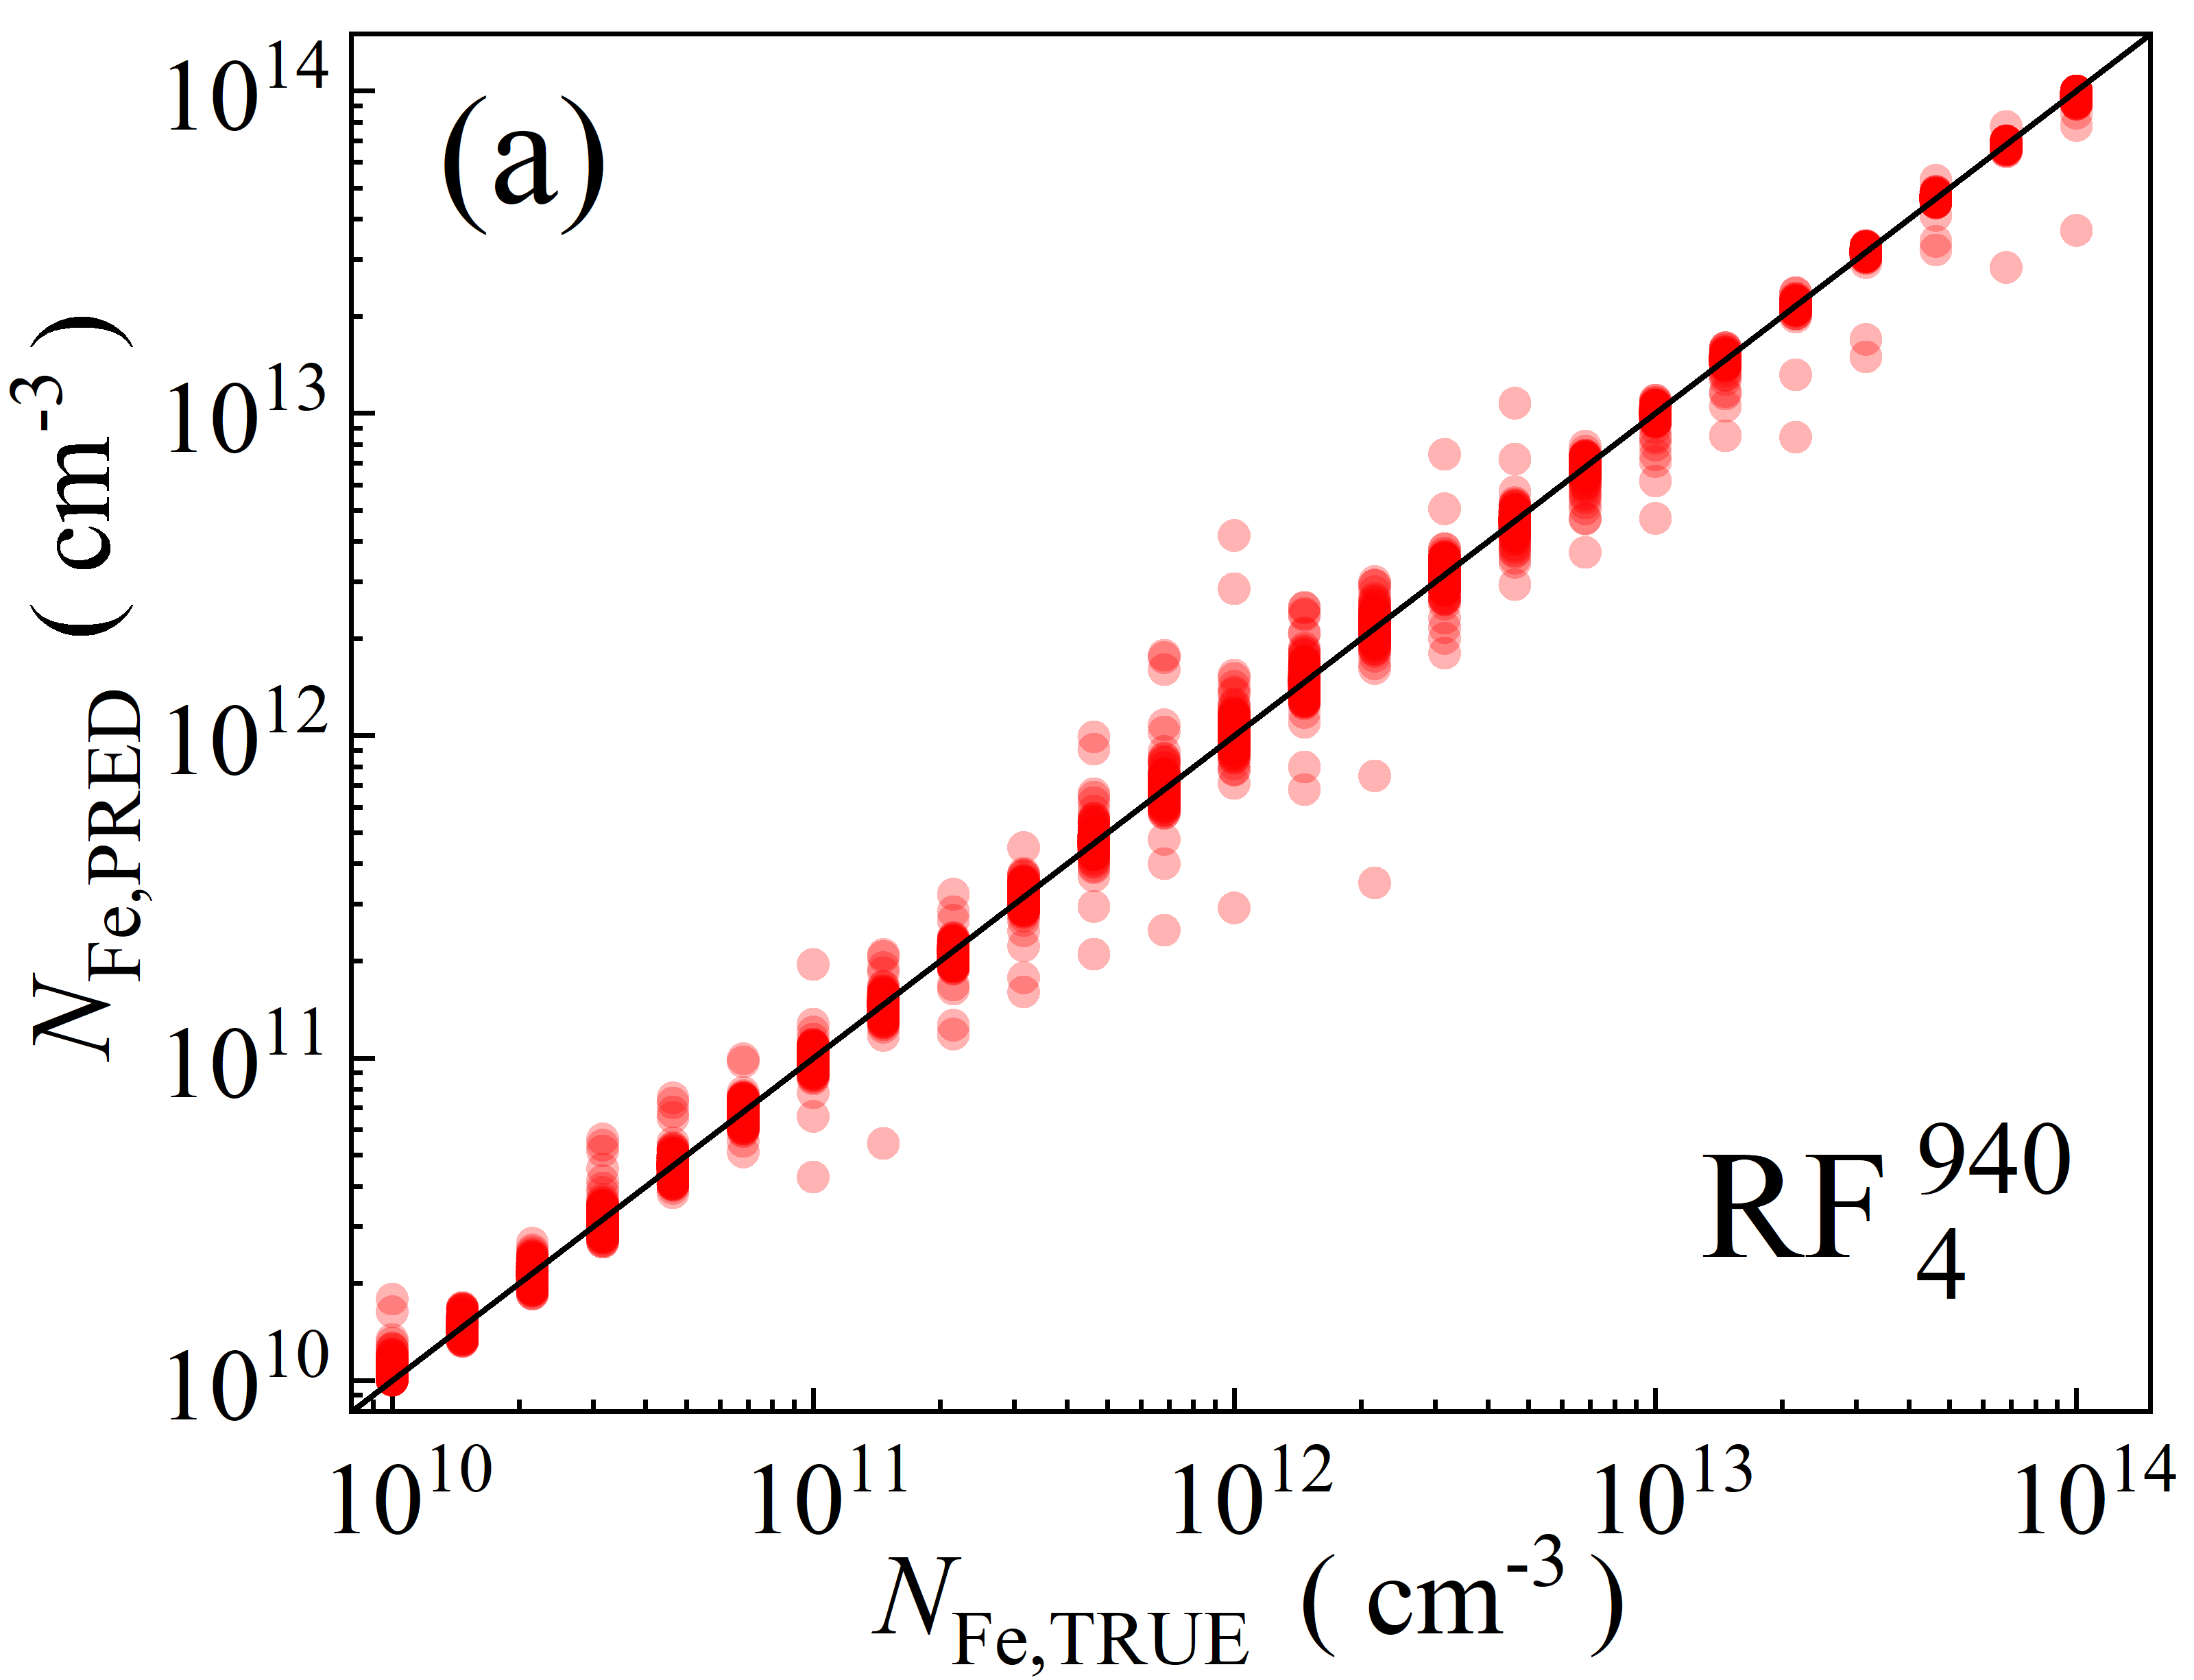
\includegraphics[width=0.4\linewidth]{Fig3a.png}
  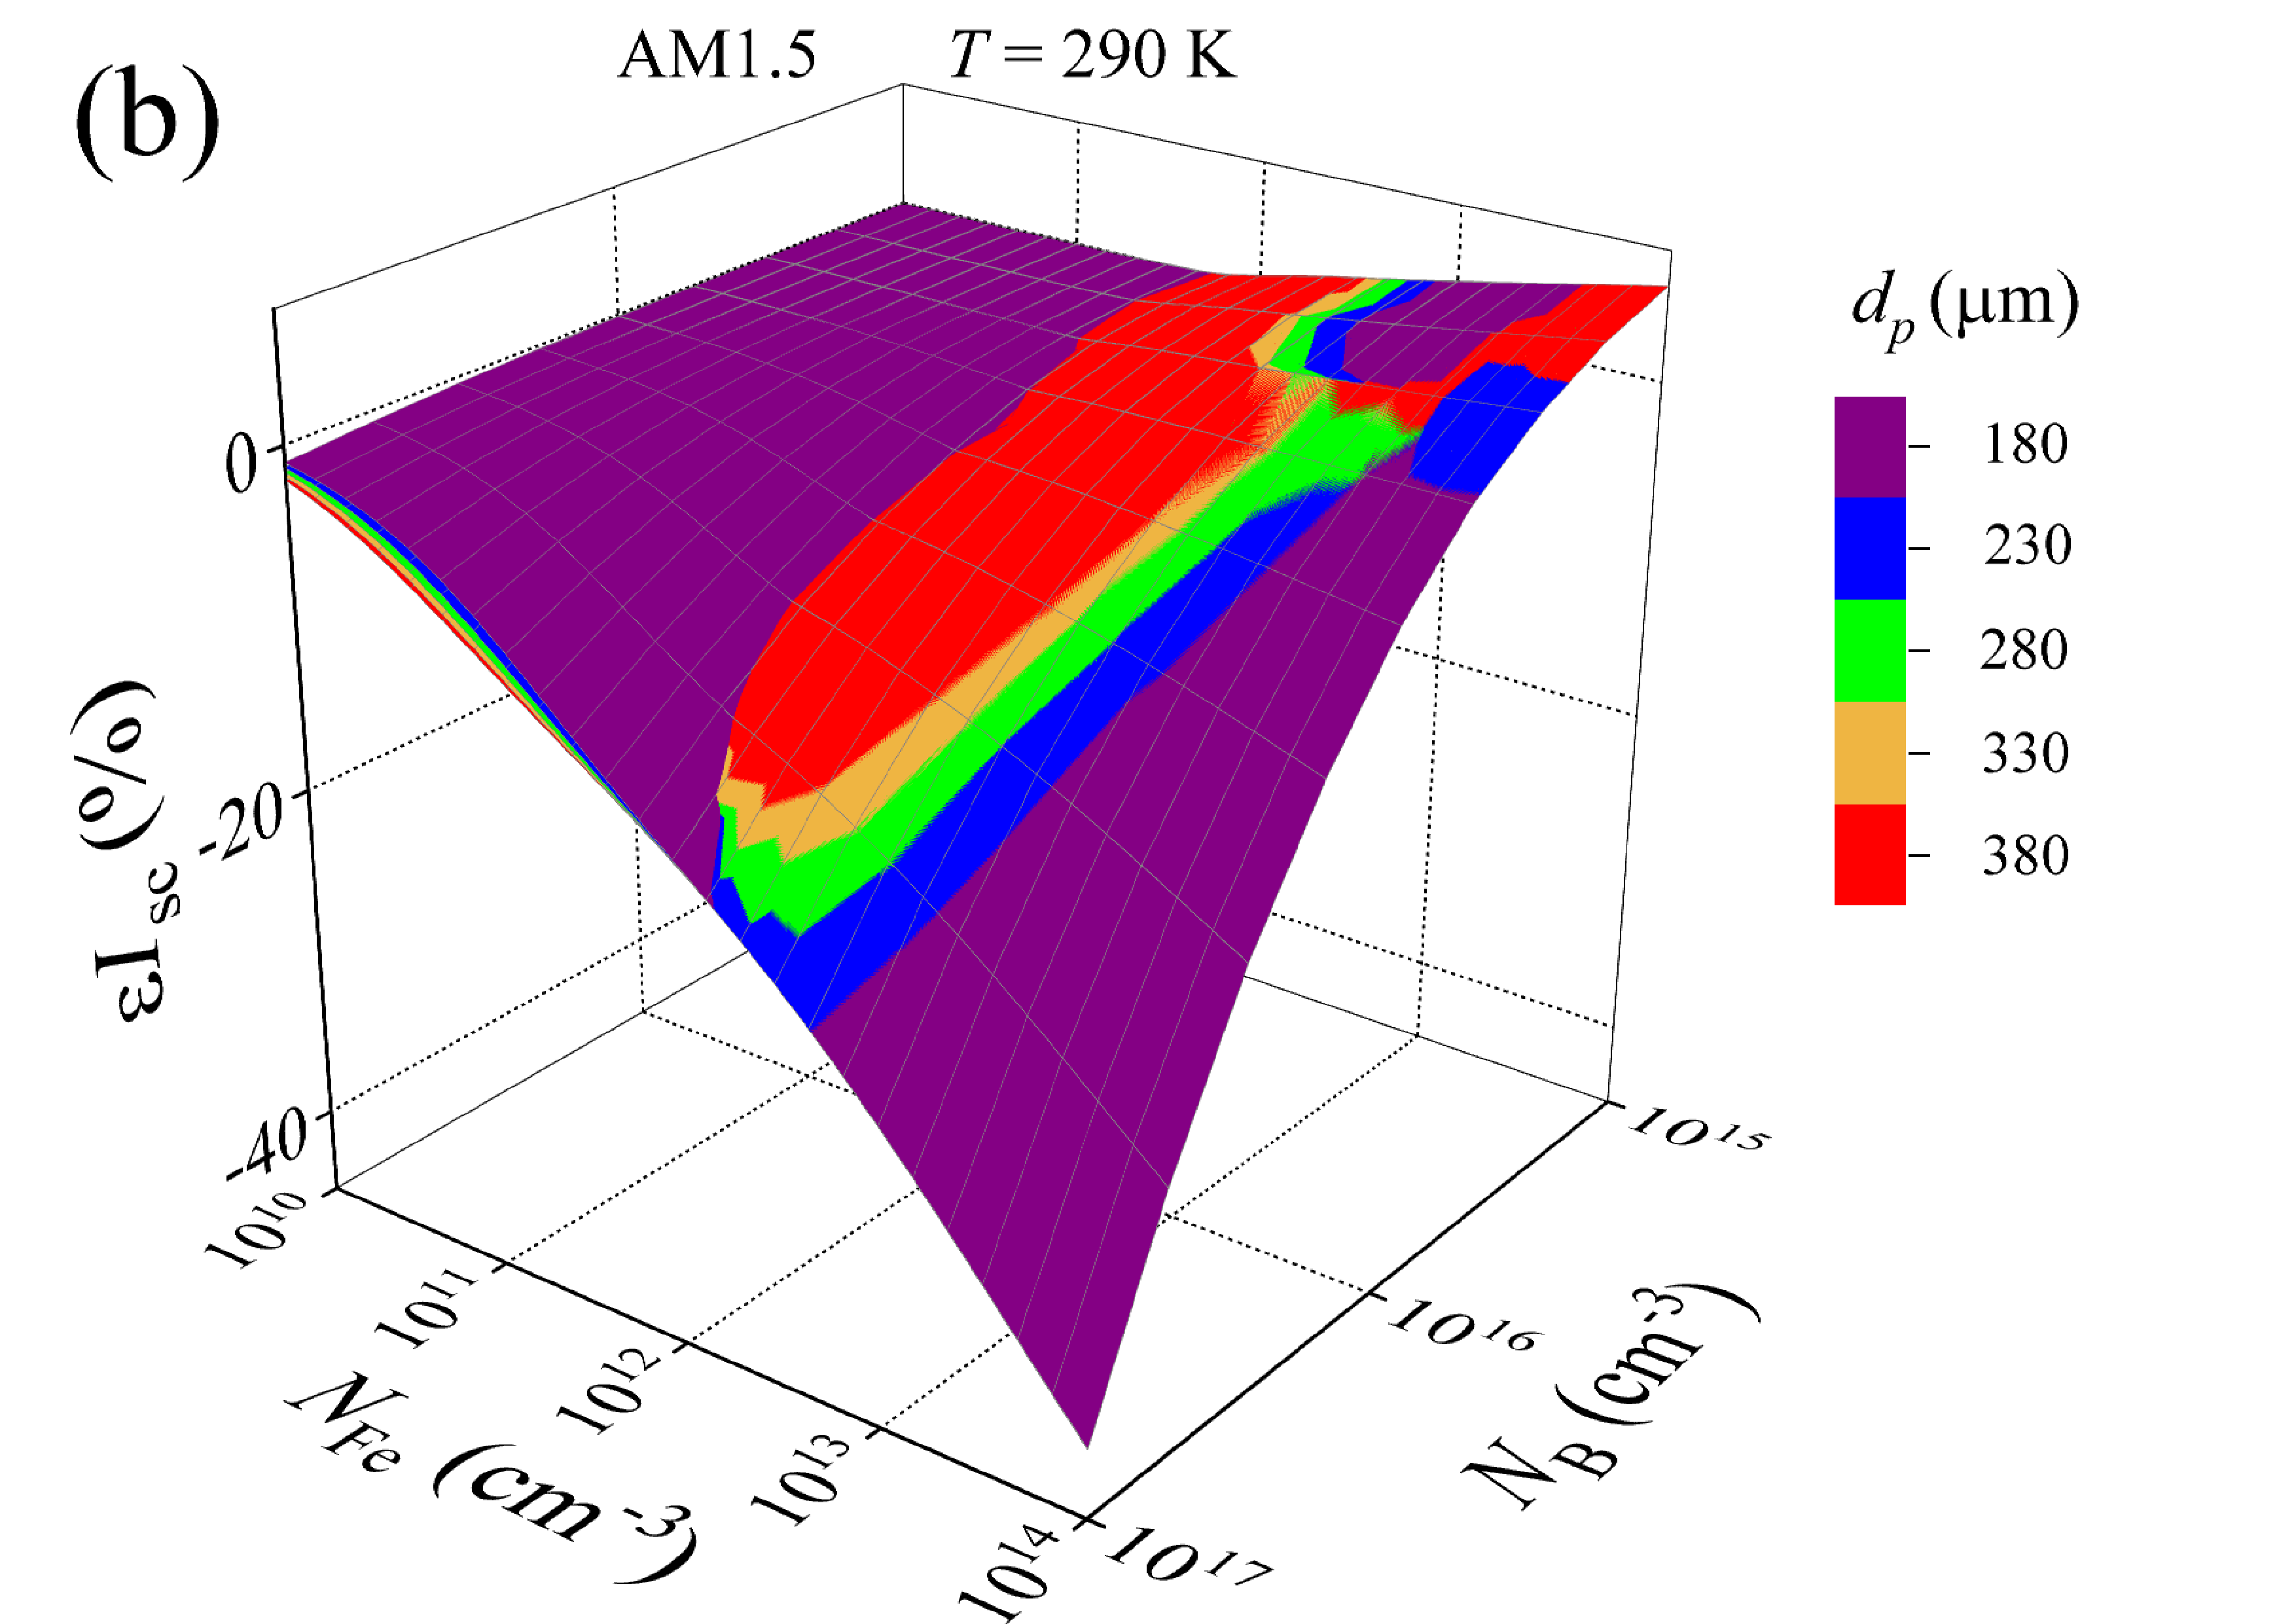
\includegraphics[width=0.4\linewidth]{Fig3b.png}
  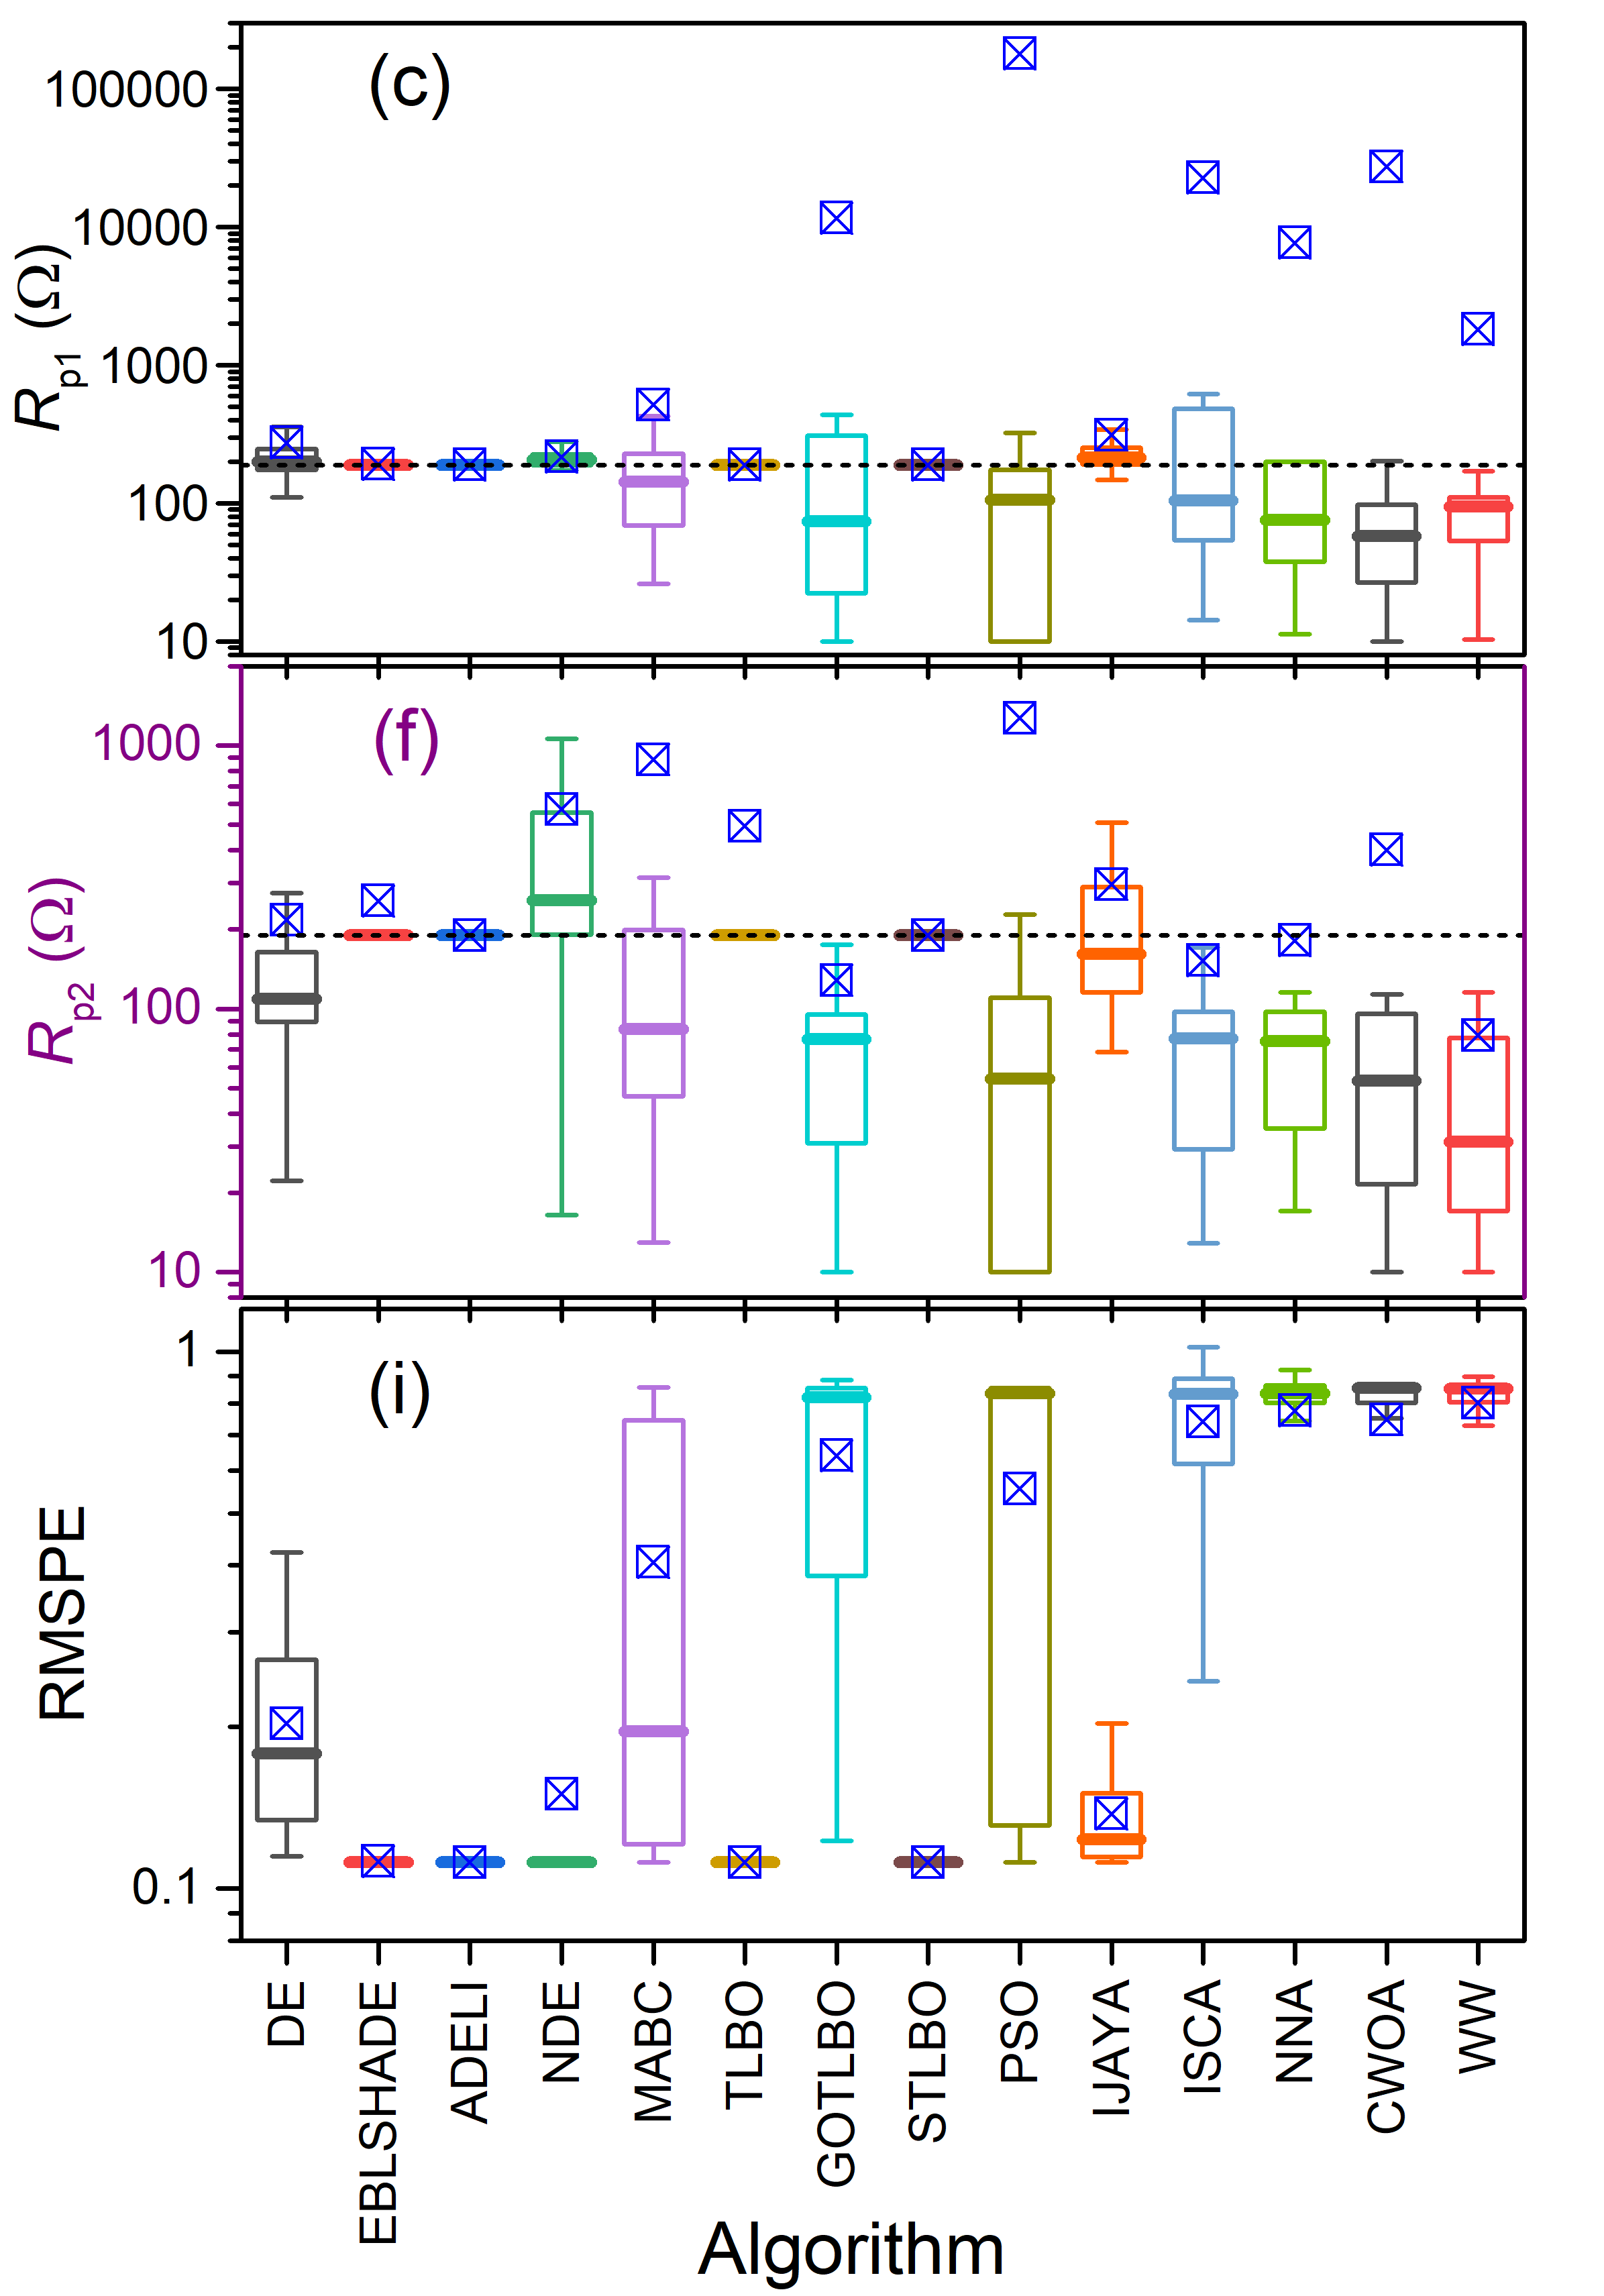
\includegraphics[width=0.4\linewidth]{Fig3c.png}
  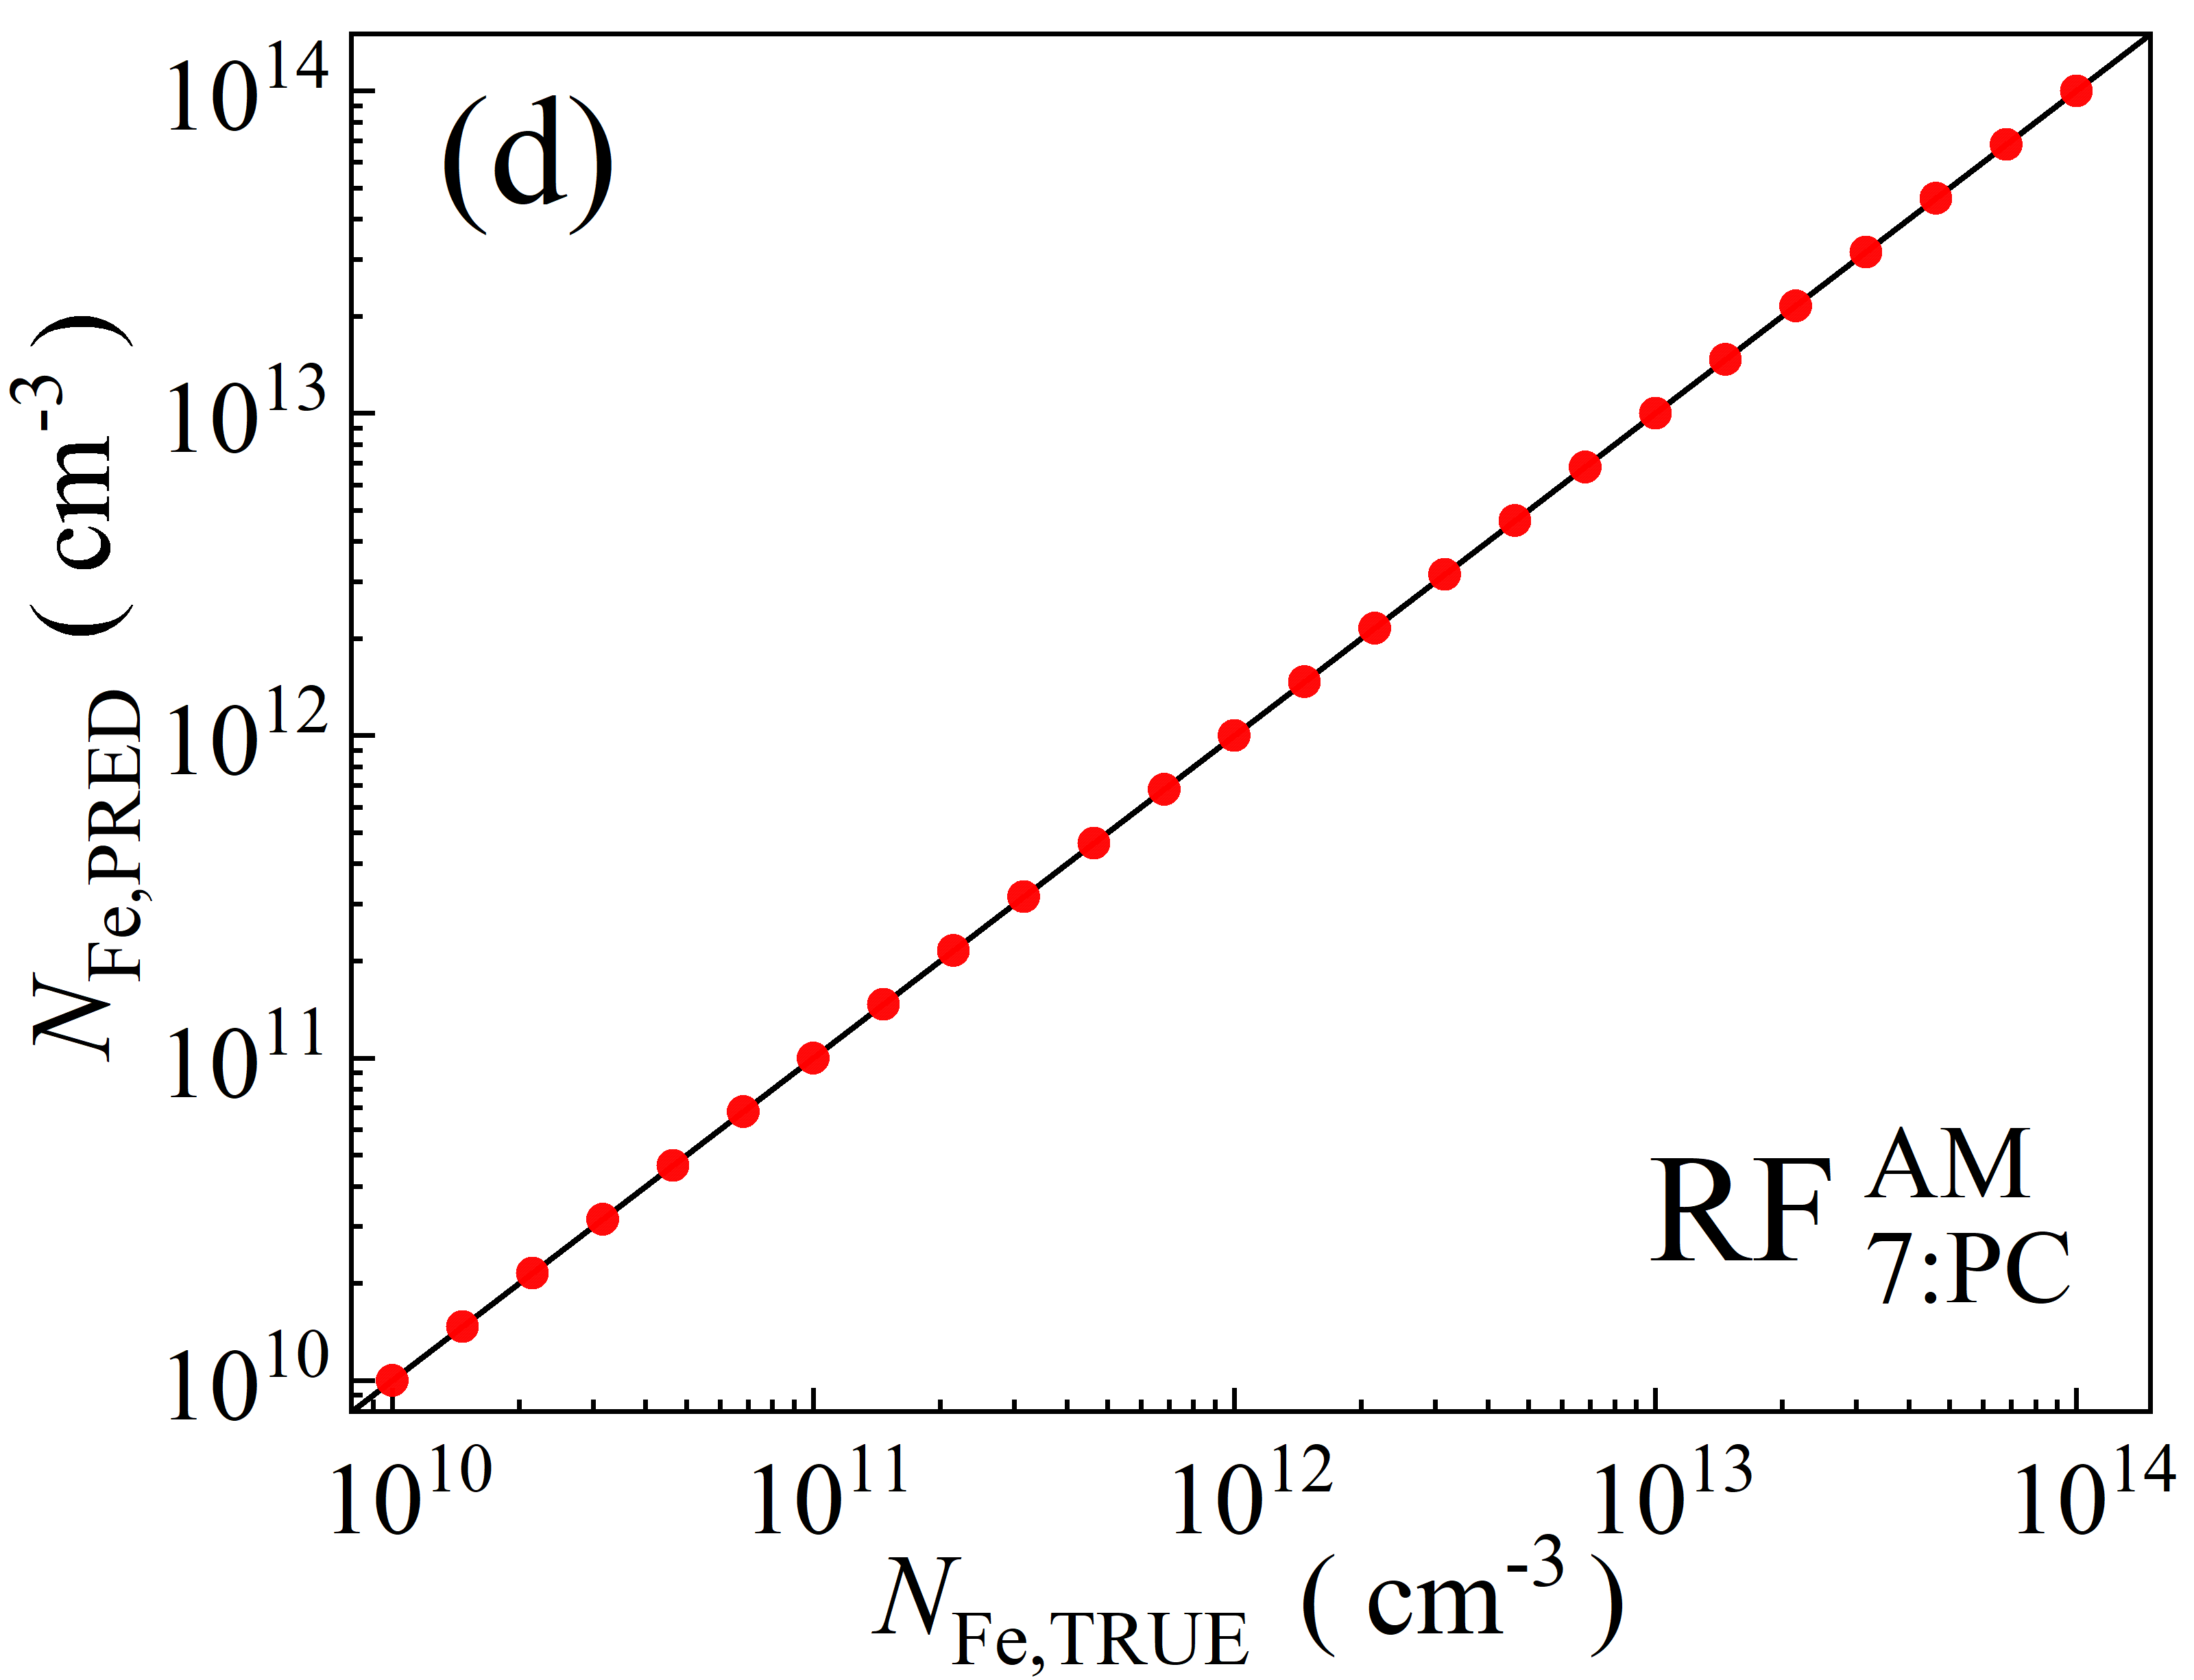
\includegraphics[width=0.4\linewidth]{Fig3d.png}
  \caption{The relationships between the concentration of FeB pairs following intense illuminations of varying intensities and the illumination duration.
  Light source: Orion (a), Osram (b), GE (c).
  Panel d highlights variations in the dissociation of pairs induced by different light sources.
  The marks are the experimental results, the lines are the fitted curves using Equation~(\ref{eqIsc}).
  $T=340$~K.}
  \label{fig3}
\end{figure}

\begin{table}
 \caption{The value of maximum concentrations of iron atoms after illumination and
characteristic dissociation time obtained by approximating experimental dependencies by Equation~(\ref{eqIsc}).
Coefficient of determination is listed as well.}
 \label{tb1}
  \begin{tabular}[htbp]{@{}ccccc@{}}
    \hline
    $W_\mathrm{ill}$~[mW] & Light source & $\tau_\mathrm{dis}$ [s] & $N_\mathrm{Fe,fit}$ [$10^{12}$~cm$^2$] & $R^2$ \\
    \hline
    750  & Orion  & $2.2\pm0.2$ & $8.6\pm0.1$ & 0.993 \\
    700  & Orion  & $2.7\pm0.2$ & $8.6\pm0.1$ & 0.995 \\
         & Osram  & $2.4\pm0.2$ & $8.6\pm0.1$ & 0.992 \\
    600  & Orion  & $3.7\pm0.2$ & $8.65\pm0.06$ & 0.998 \\
         & Osram  & $3.0\pm0.2$ & $8.69\pm0.08$ & 0.995 \\
    500  & Orion  & $5.5\pm0.2$ & $8.65\pm0.04$ & 0.999 \\
         & Osram  & $4.5\pm0.1$ & $8.7\pm0.1$ & 0.998 \\
    400  & Orion  & $8.8\pm0.3$ & $8.74\pm0.06$ & 0.998 \\
         & Osram  & $6.1\pm0.2$ & $8.63\pm0.08$ & 0.997 \\
         & GE  & $3.6\pm0.3$ & $8.7\pm0.1$ & 0.996 \\
    300  & Orion  & $15.7\pm0.6$ & $8.6\pm0.1$ & 0.998 \\
         & Osram  & $12.4\pm0.1$ & $8.69\pm0.02$ & 0.999 \\
         & GE  & $6.5\pm0.2$ & $8.69\pm0.05$ & 0.998 \\
    200  & Orion  & $35\pm3$ & $8.5\pm0.3$ & 0.998 \\
         & Osram  & $24\pm1$ & $8.6\pm0.1$ & 0.999 \\
         & GE  & $15.1\pm0.5$ & $8.7\pm0.1$ & 0.999 \\
    \hline
  \end{tabular}
\end{table}




%solar simulator setup FeBKin2019
%white light illumination FeBJAP2005

Reassessing iron–gallium recombination activity in silicon \cite{Le2024}

AIPAdv 3 082124 \cite{FeBStrongIll}

Effect of Dopant Compensation on the Behavior of Dissolved
Iron and Iron-Boron Related Complexes in Silicon InterJPhotoener 2015 154574 \cite{Zhu2015}

JApplPhys 116 024503 \cite{FeBAssJAP2014}

PhysStatSolA 216 1900253 \cite{FeBKin2019}

PhysStatSolRRL 15 2100520 \cite{Sun2021}

PR ApplPhysLett 85 p5227 5229 \cite{FeBLight2}

PR JApplPhys 98 083509 \cite{FeBJAP2005}

SolStPhenom 242 p230 \cite{lauer2016}

JApplPhys 95 p1021 \cite{Macdonald2004}

PR PhysStSolRRL 6 p1 \cite{FeMethod2012}






\subsection{Carrier generation rate estimation}\label{SecG}

\begin{figure}
\centering
  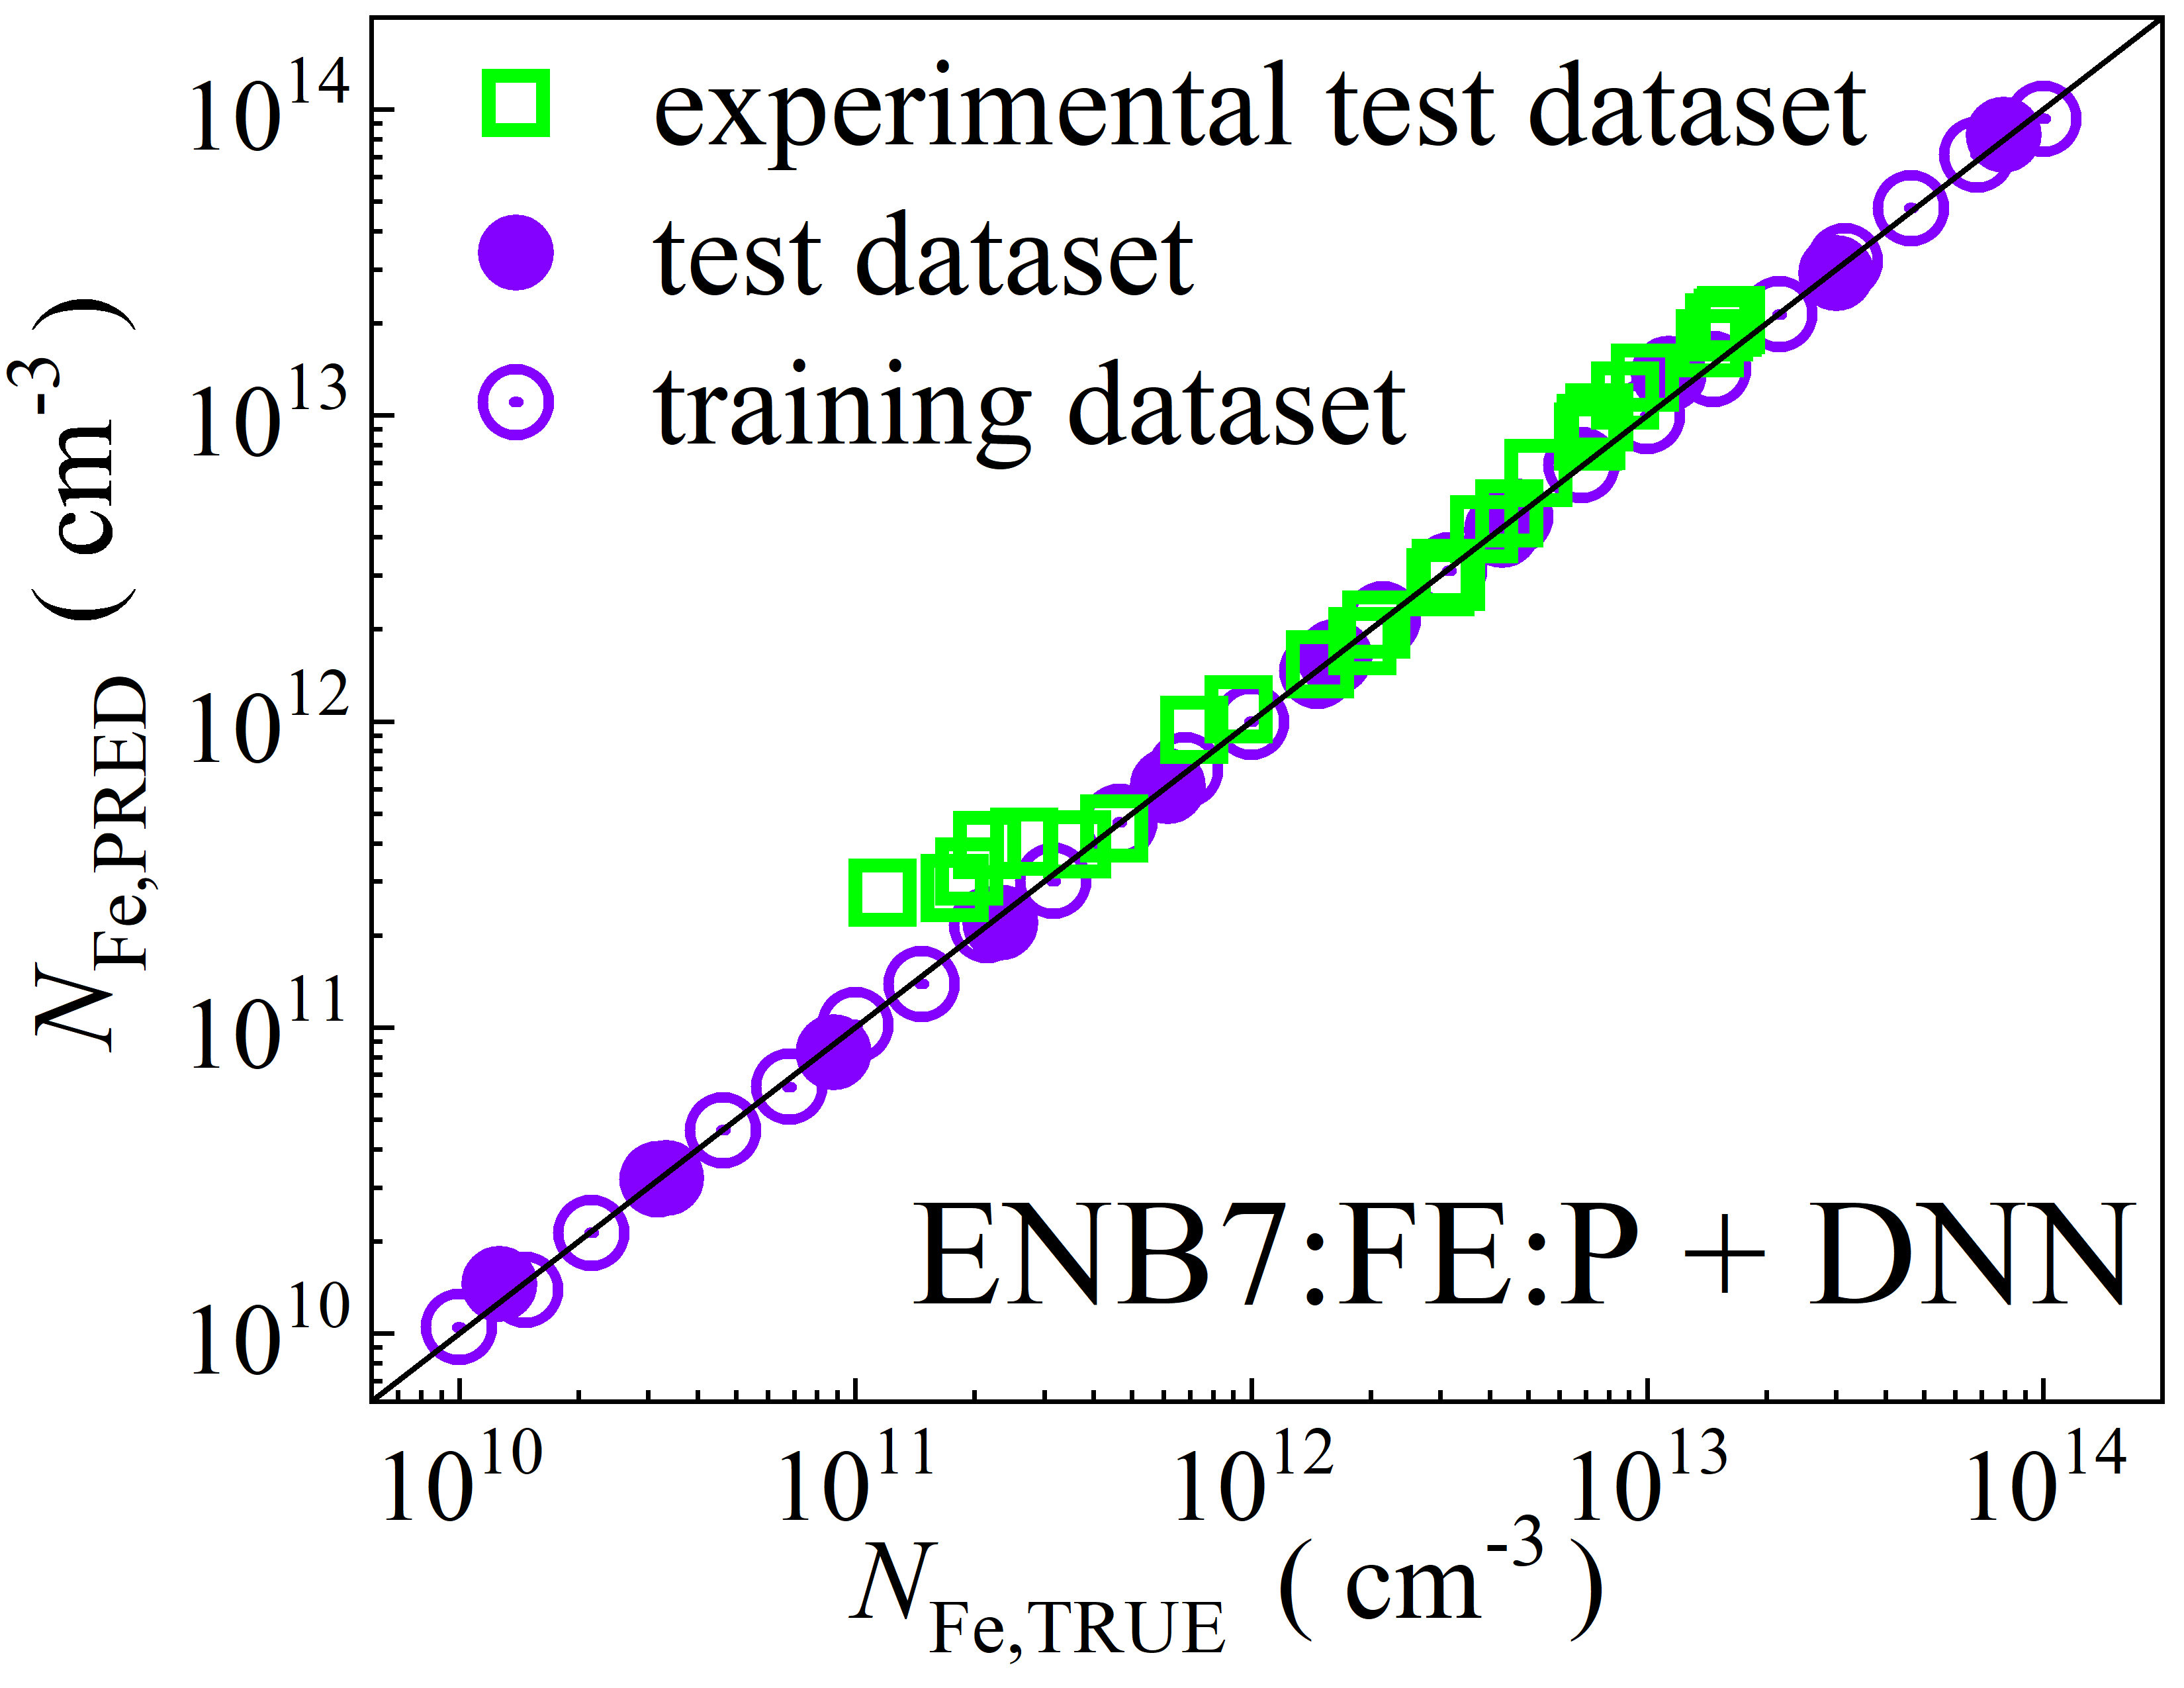
\includegraphics[width=0.4\linewidth]{Fig4a.png}
  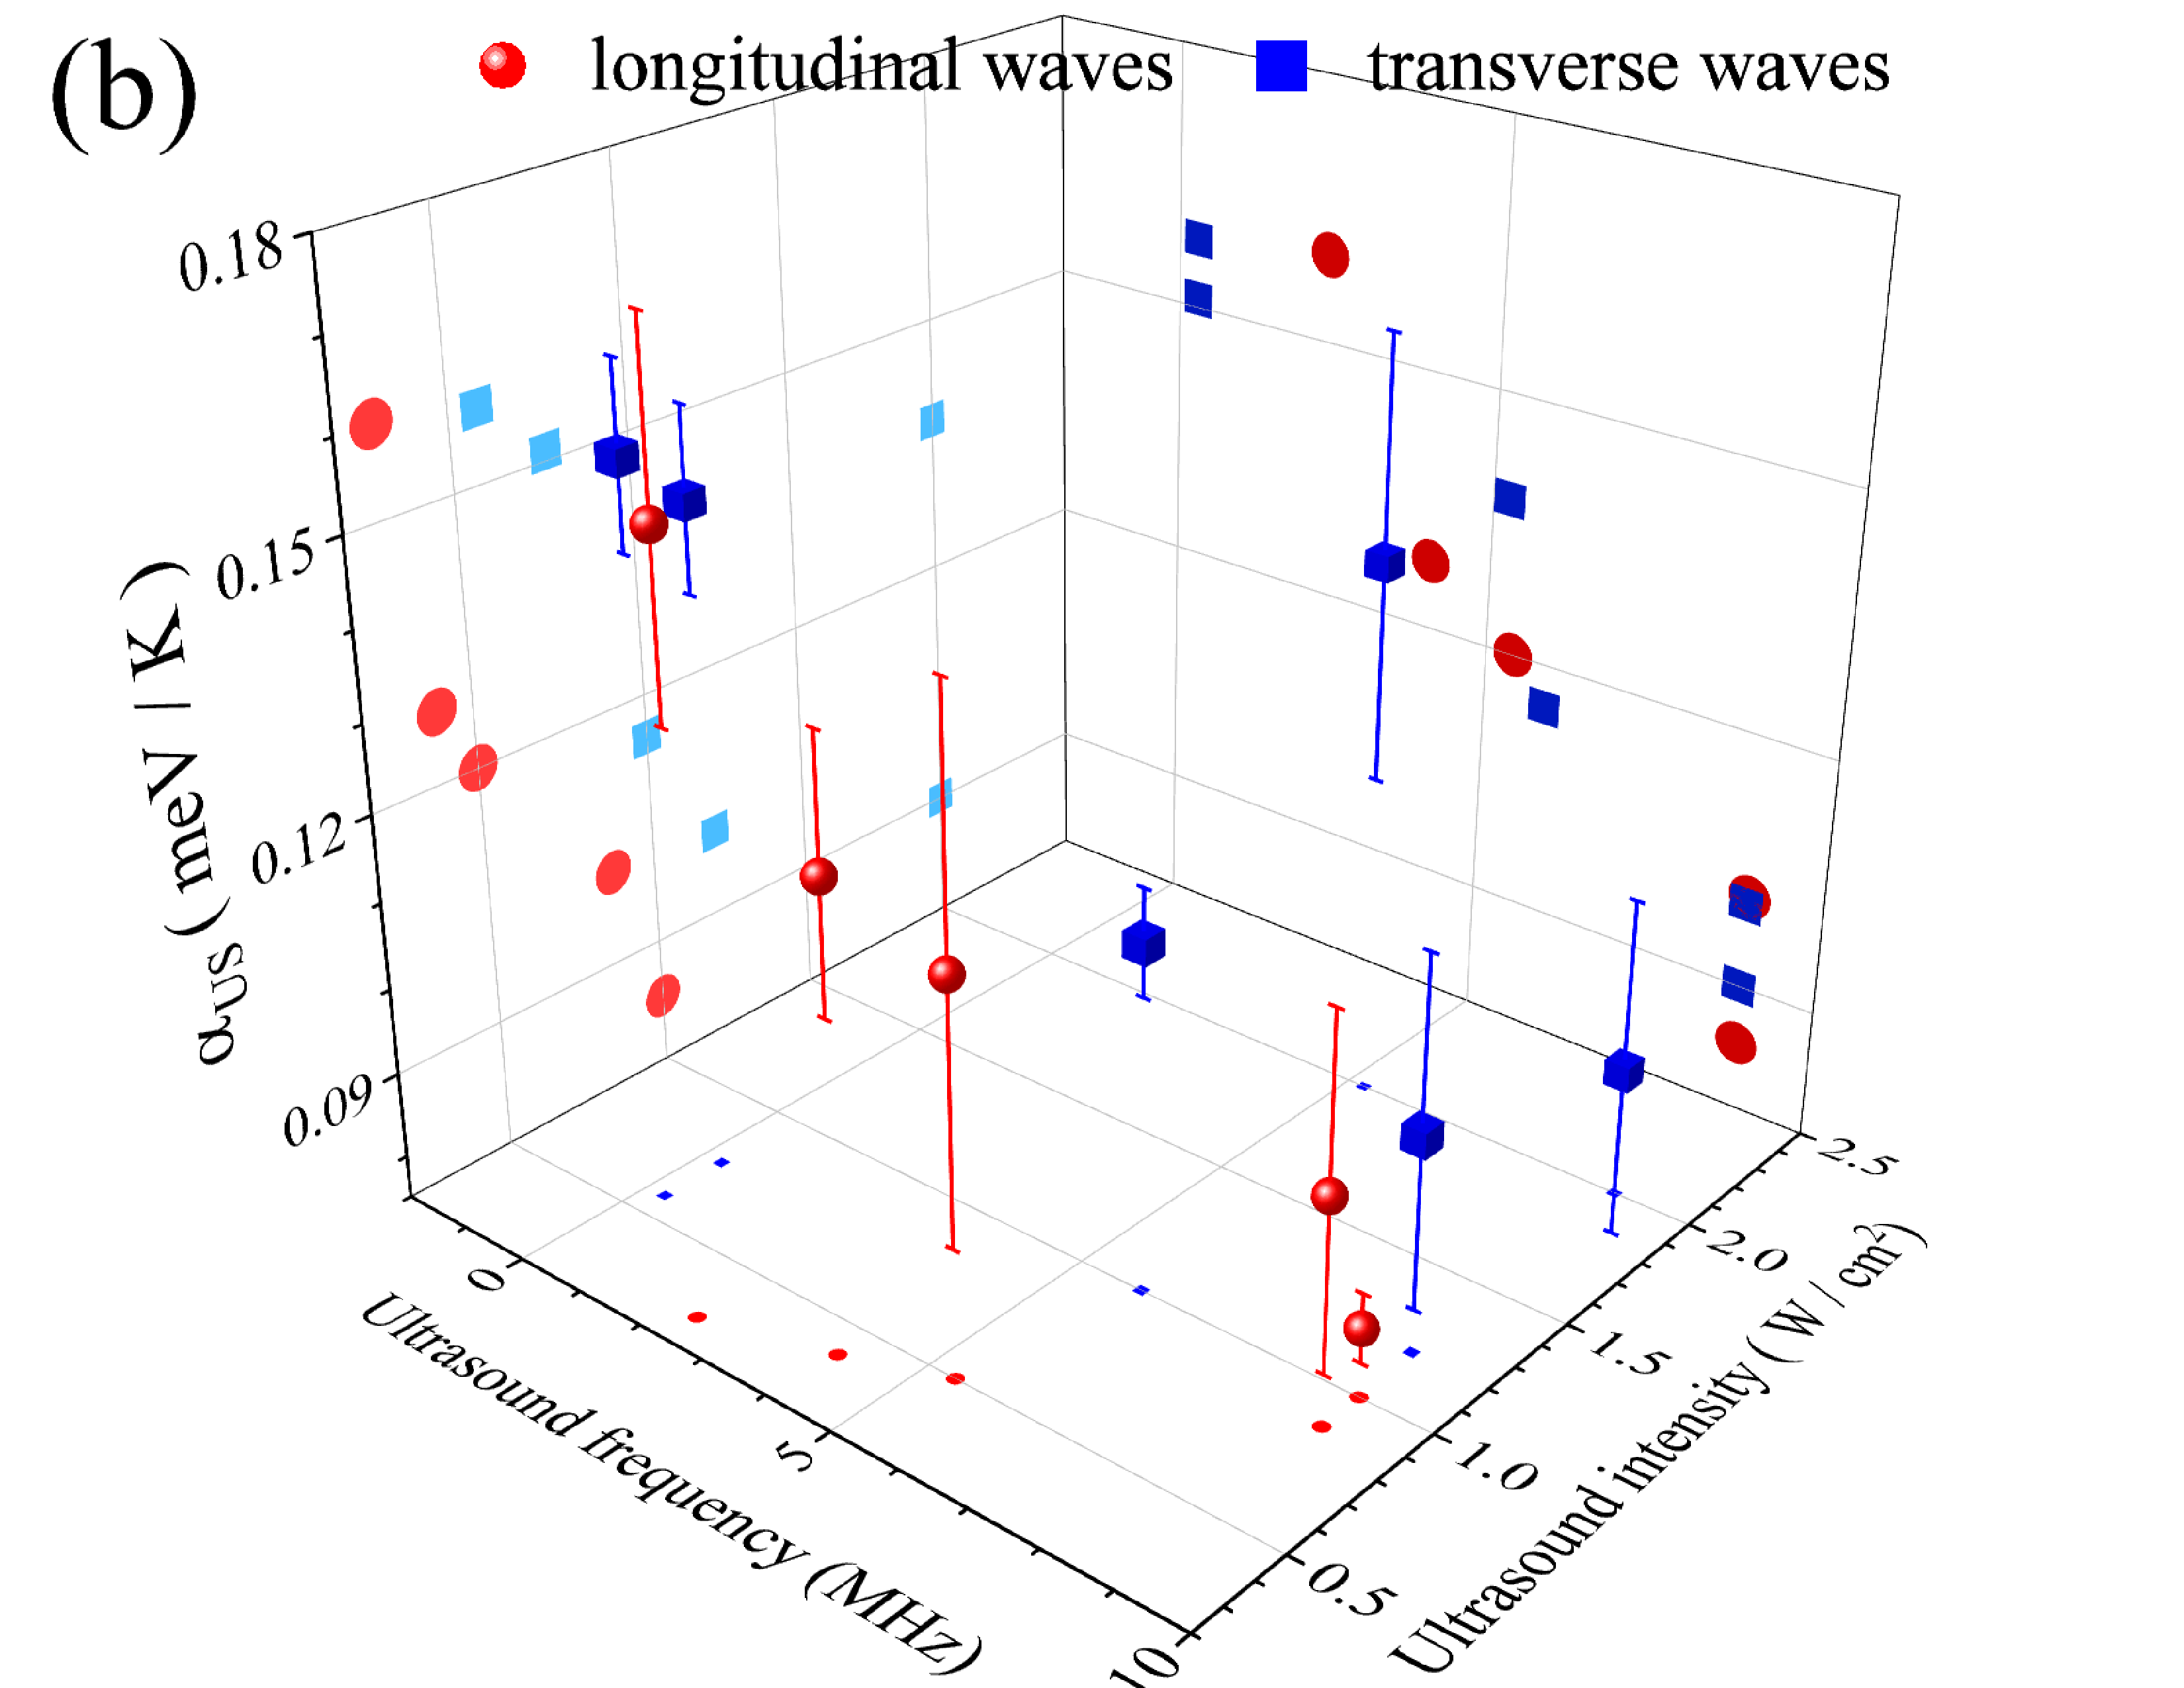
\includegraphics[width=0.4\linewidth]{Fig4b.png}
  \caption{
  The spectra of sample illumination in the case of using different light sources
  with the same integrated intensity $W_\mathrm{ill}=400$~mW (panel a) and a single source (Osram)
 at various $W_\mathrm{ill}$ values (panel b).
 The inset shows photos of light sources.
}
  \label{fig4}
\end{figure}

A part of the radiation especially in the near infrared region of the spectrum is modified by infrared transparency of the reflector and by absorption in
the plexiglass window. \cite{Libra2017}

%photon flux spectral density I(λ)

$d_\mathrm{eff}$ \cite{Bowden2007}

$A_\mathrm{bb}$ \cite{Schaefer2018}

$\alpha_\mathrm{bb}$, refractive index $n$ \cite{Green2022}

$\alpha_\mathrm{fca}$ \cite{SiFCA}


\begin{figure}
\centering
  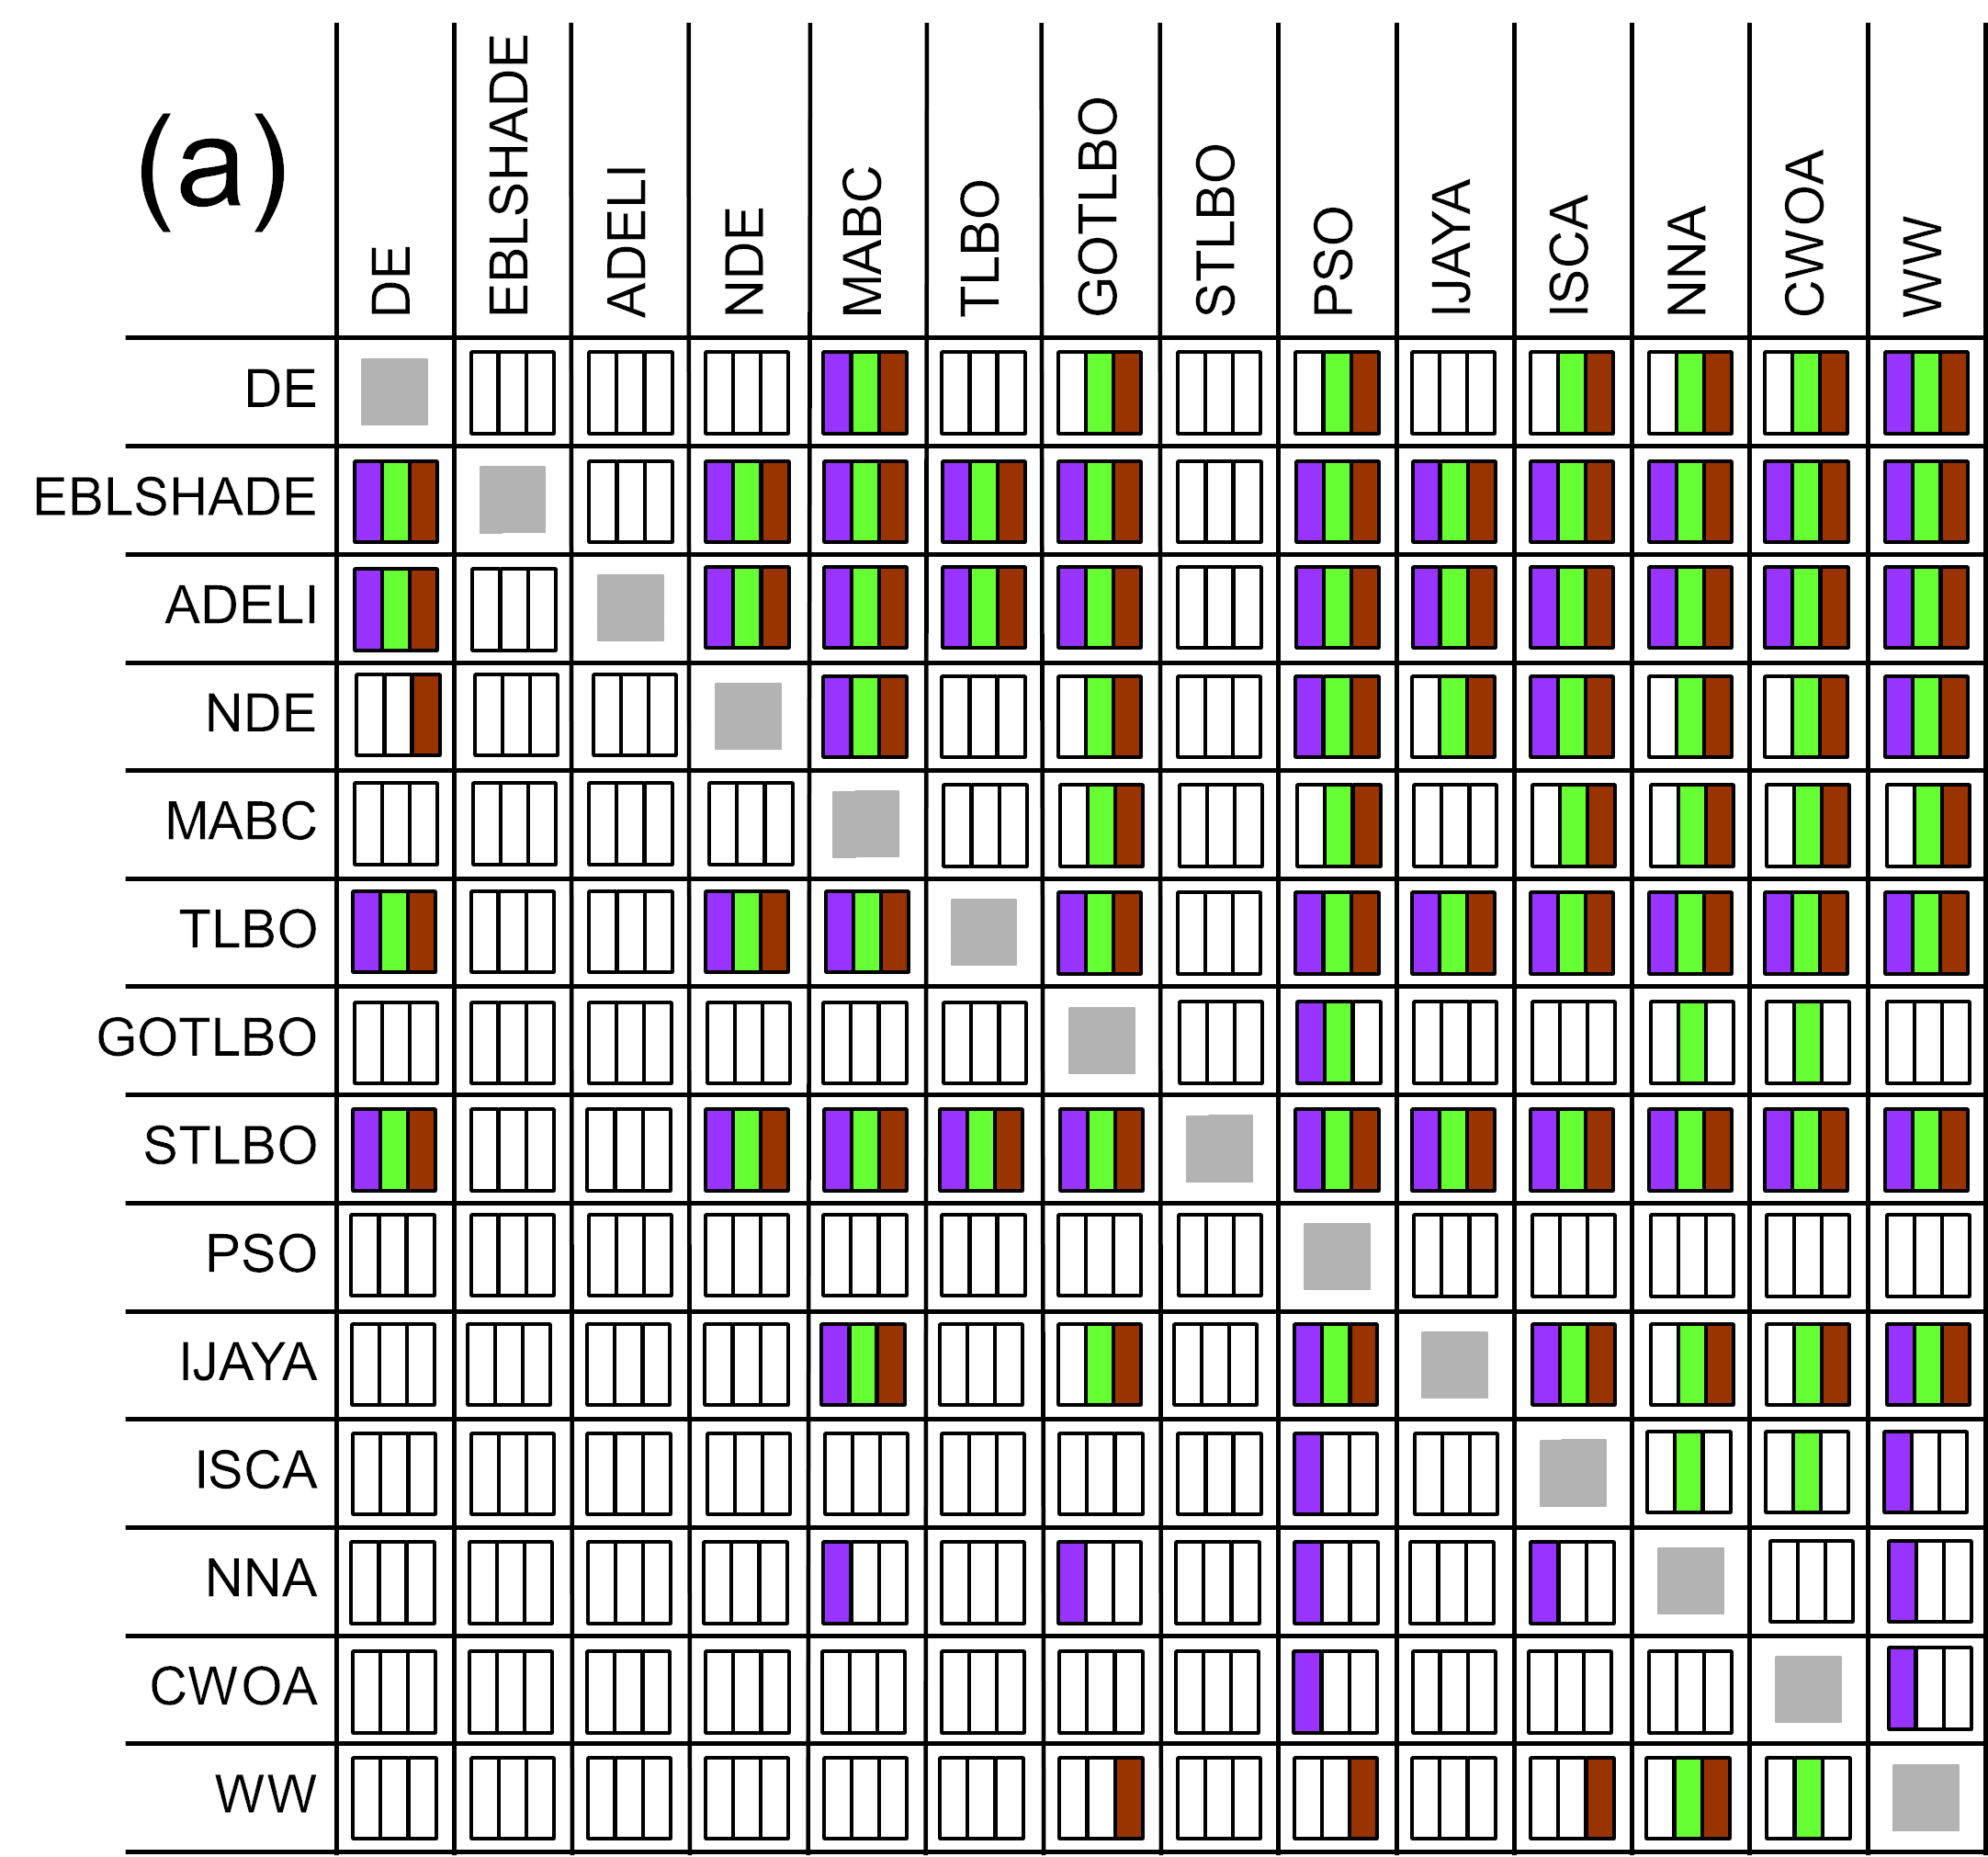
\includegraphics[width=0.4\linewidth]{Fig5a.png}
  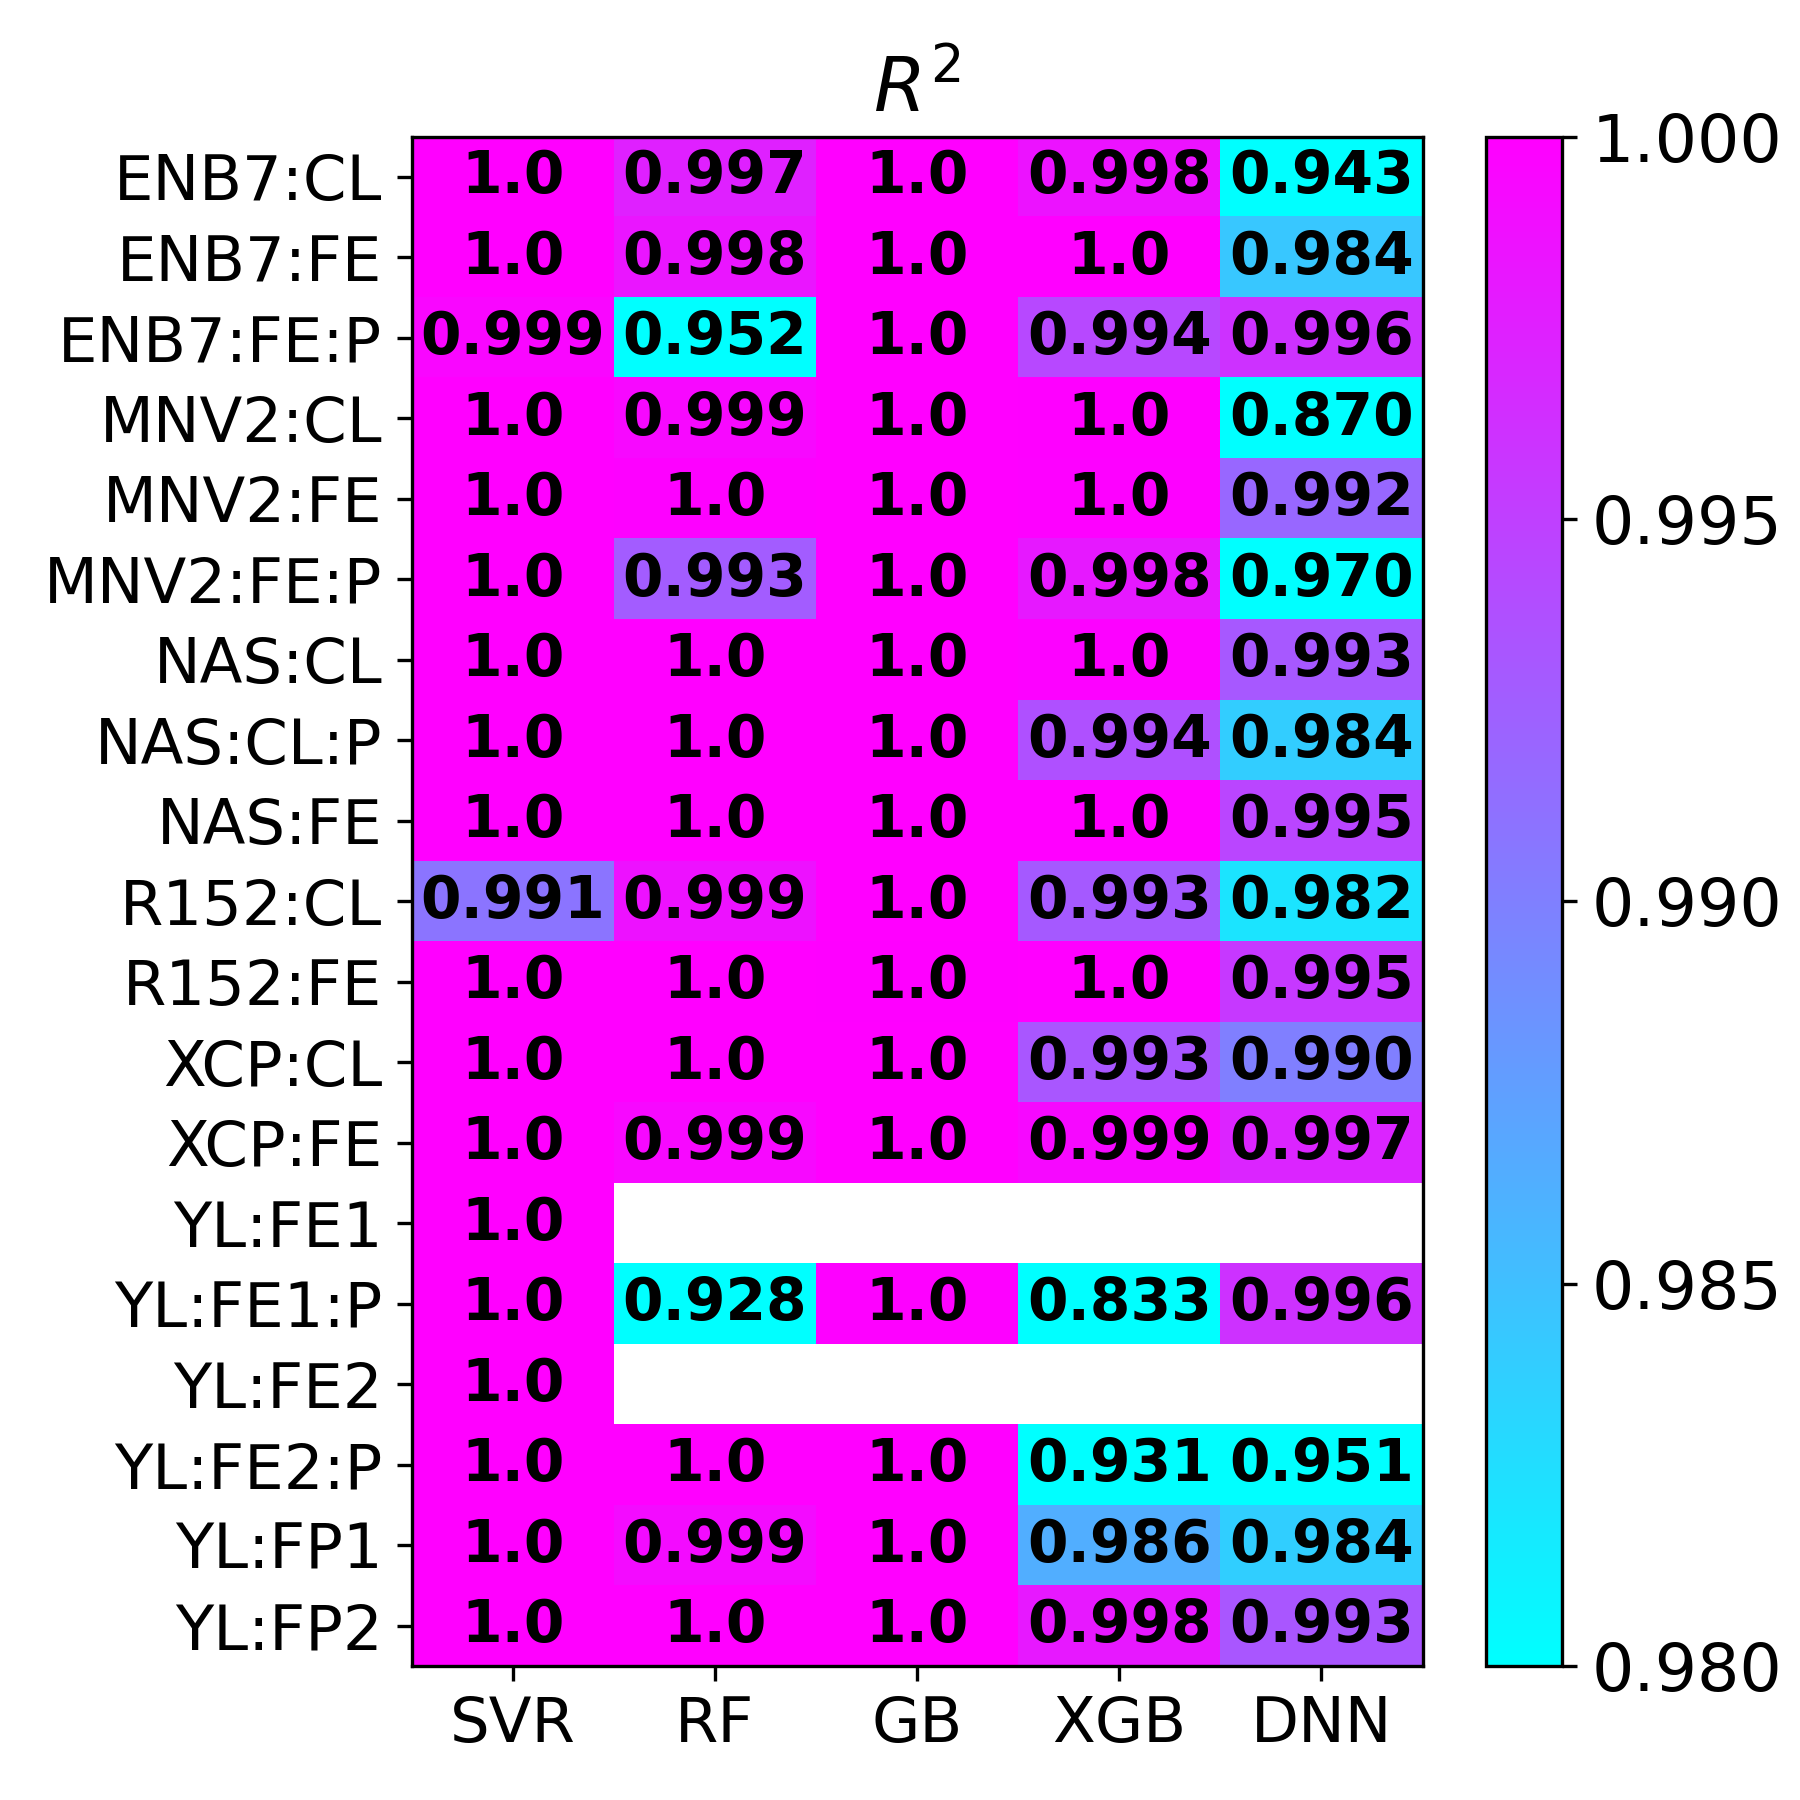
\includegraphics[width=0.4\linewidth]{Fig5b.png}
  \caption{
  (a) Photon flux spectral density (left axis, solid line) and carrier generate rate spectral density (right axis, dashed line).
  Orion light source, $W_\mathrm{ill}=400$~mW.
  (b) Dependencies of carrier generation rate on illumination intensity for different light sources.
  }
  \label{fig5}
\end{figure}




\subsection{Effect of illumination spectrum on FeB pair decay}\label{SecLast}




\begin{figure}
\centering
  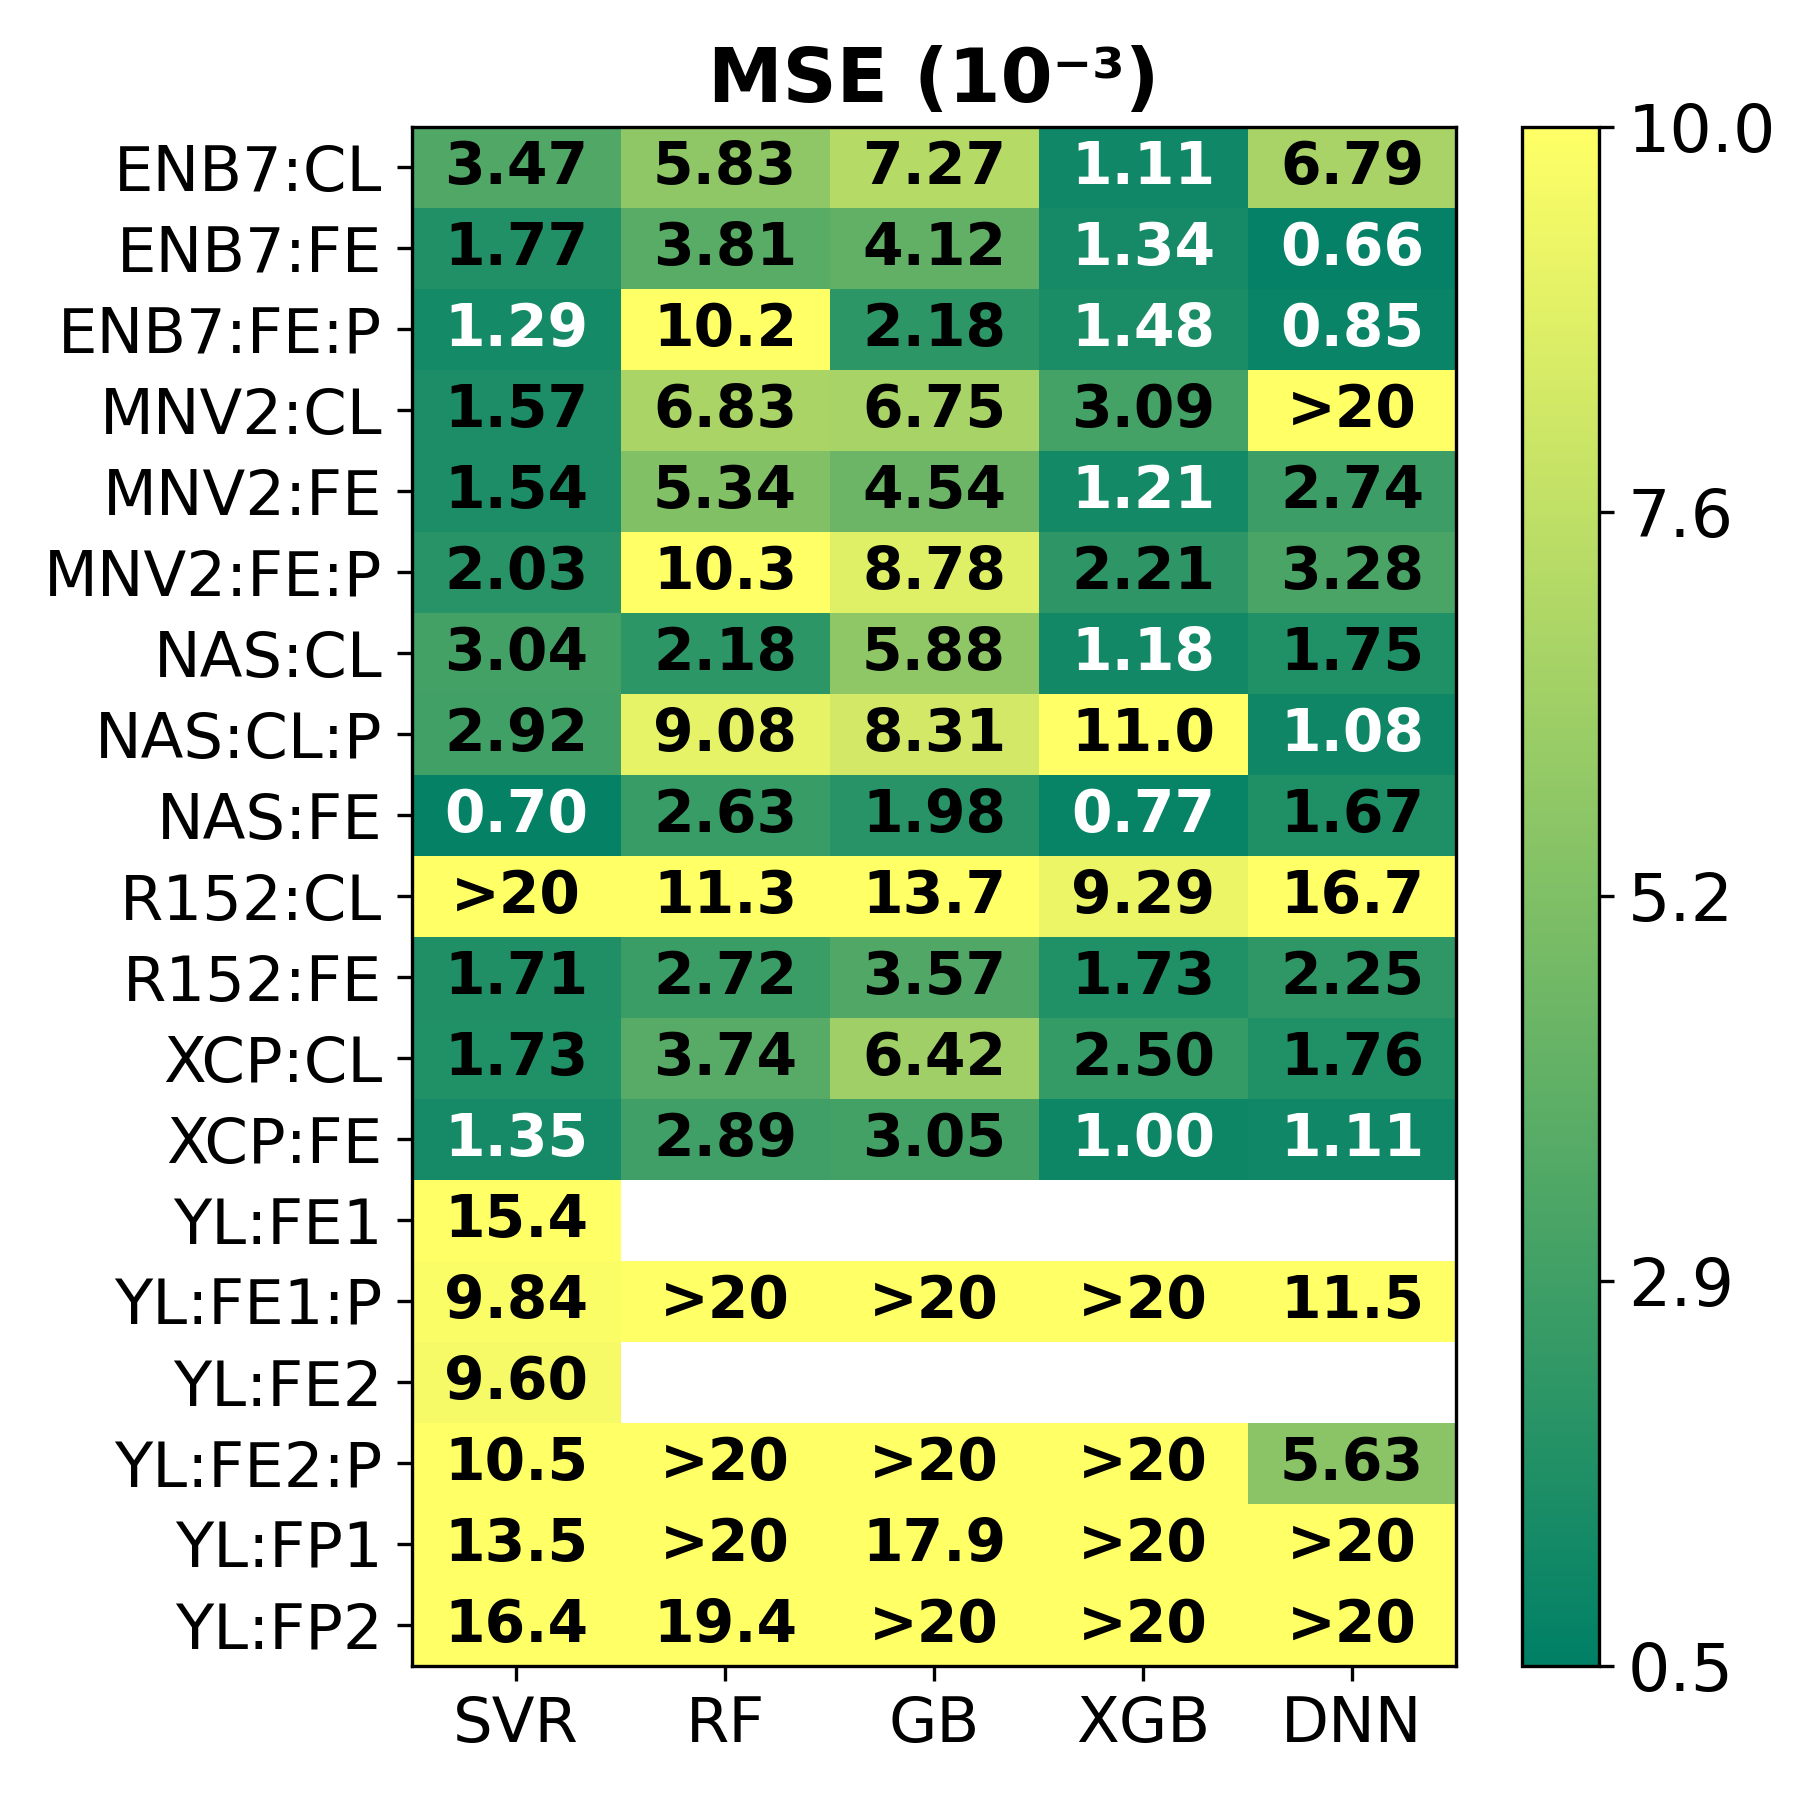
\includegraphics[width=0.4\linewidth]{Fig6a.png}
  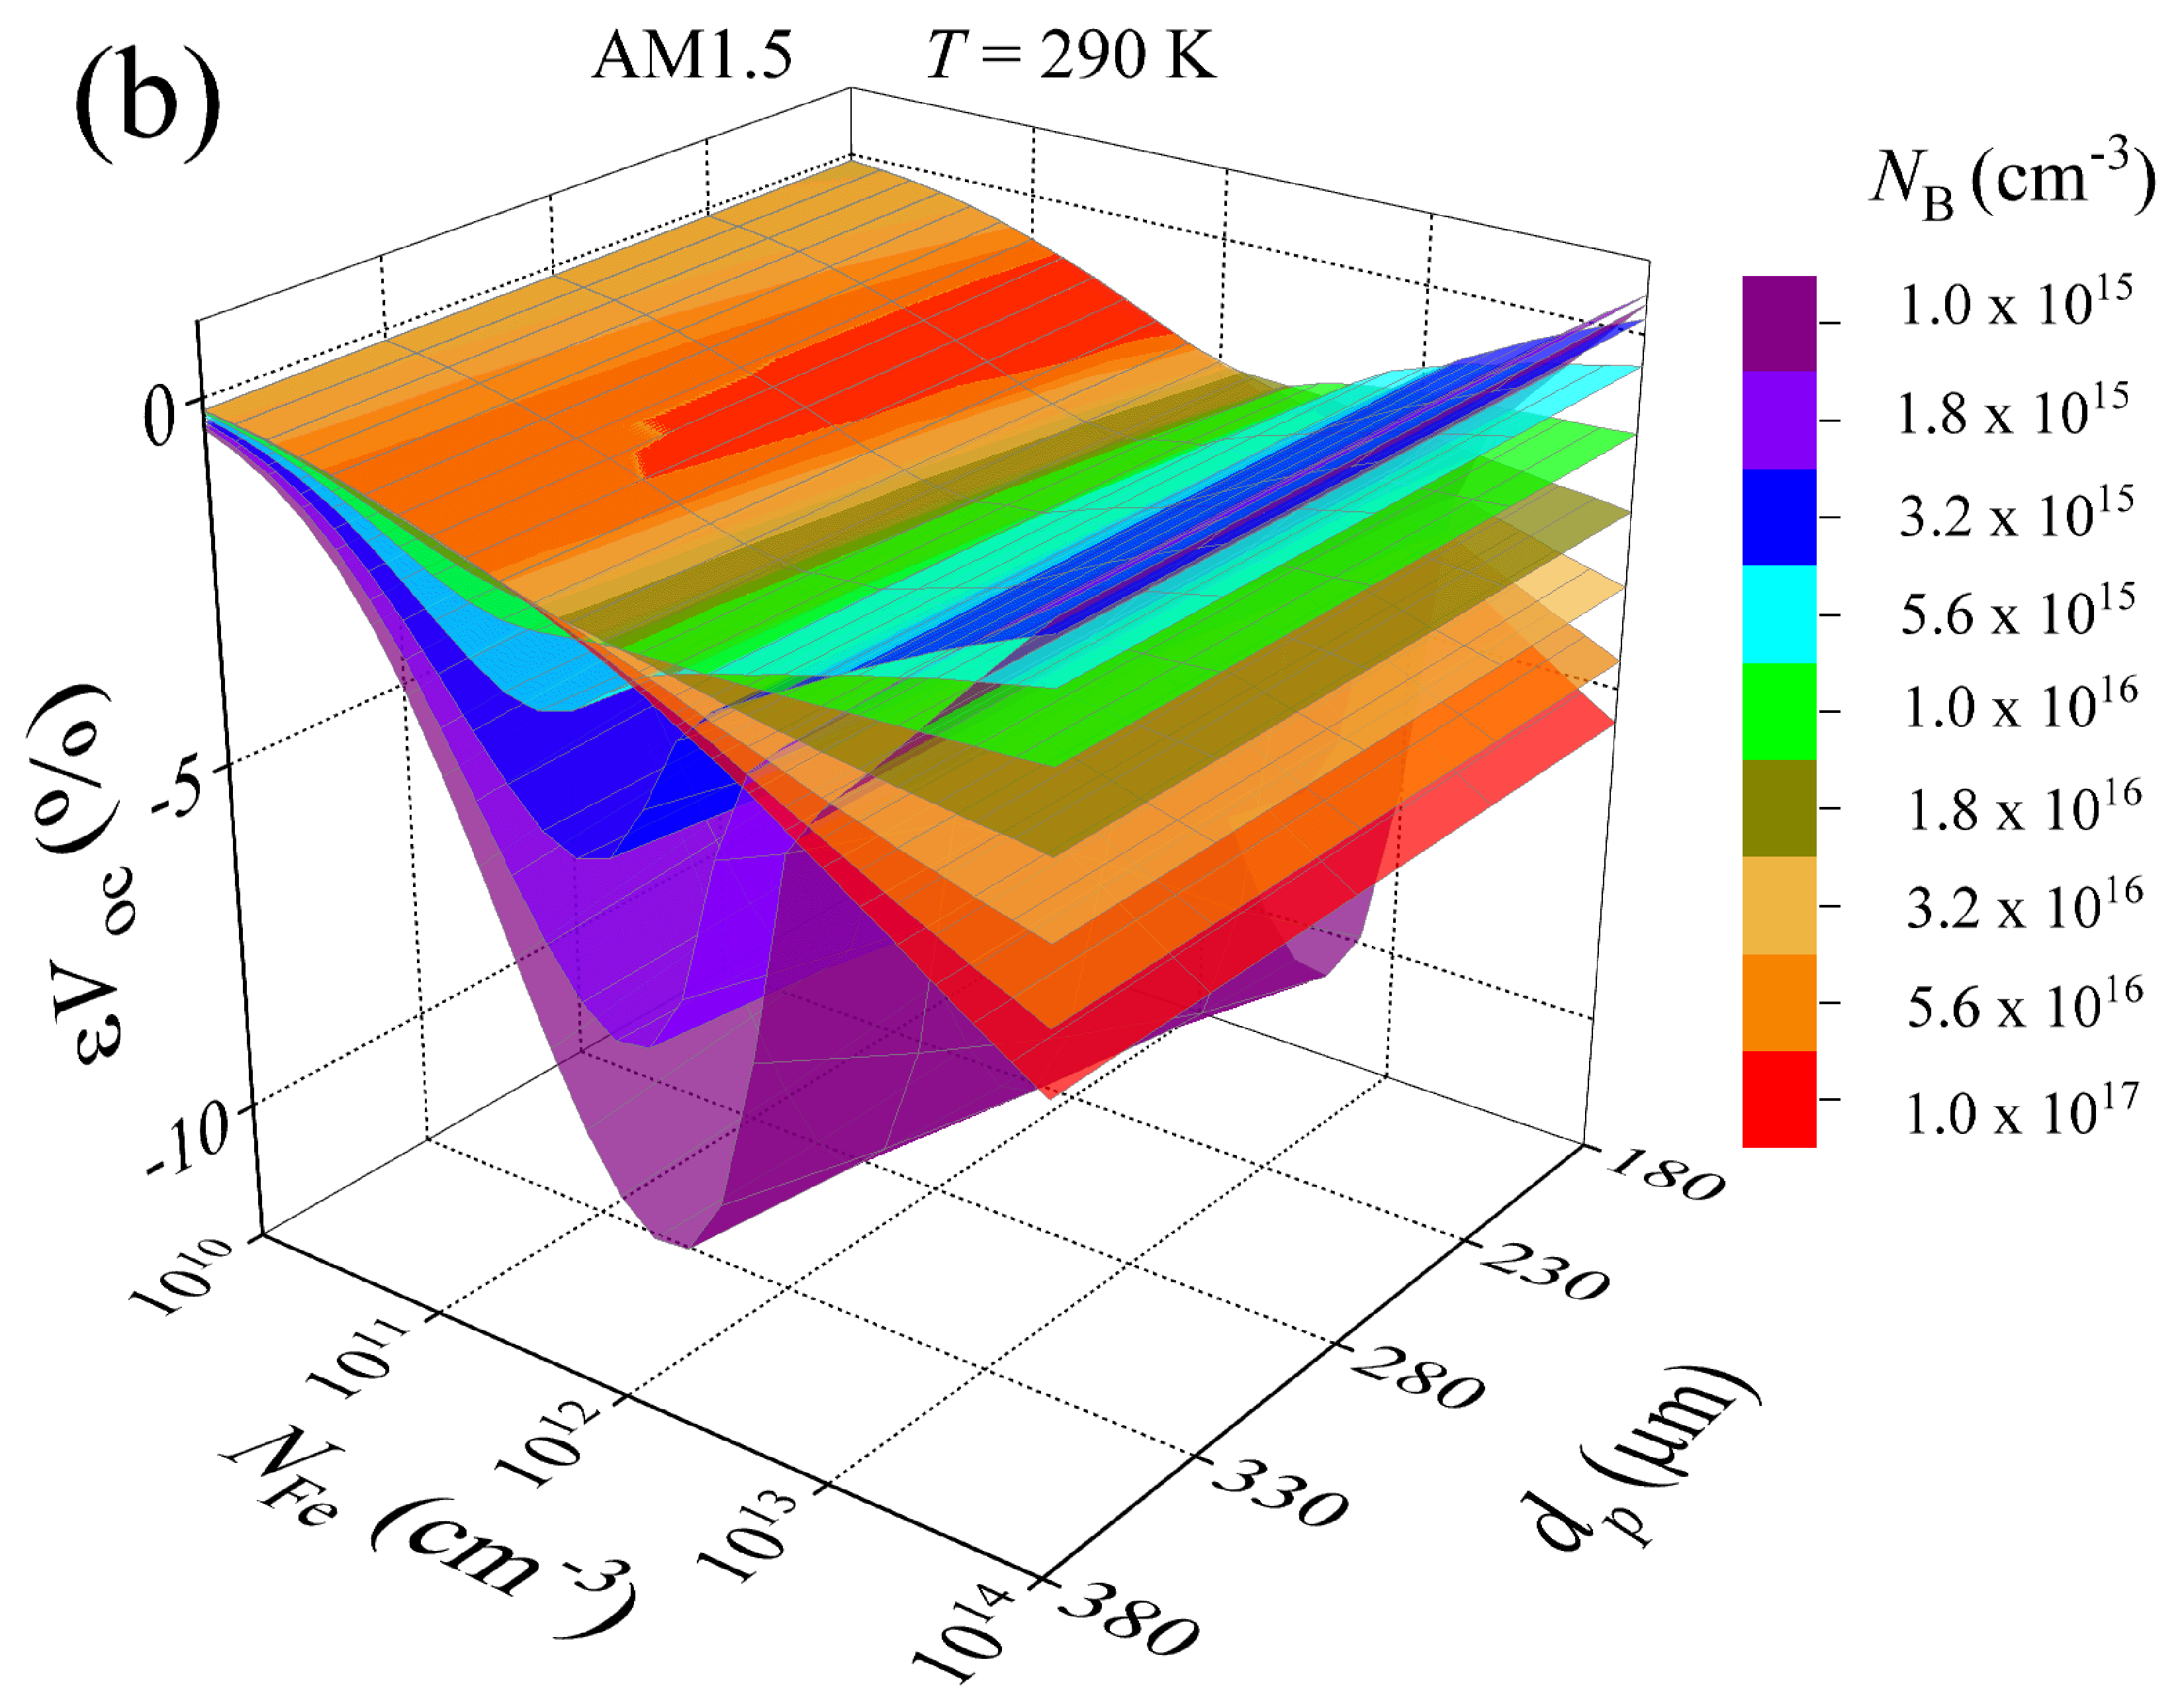
\includegraphics[width=0.4\linewidth]{Fig6b.png}
  \caption{
  (a) FeB pair dissociation rate plotted as $R_d\cdot N_\mathrm{FeB}^2$ over the light induced
  generation rate. The solid lines show the quadratic dependence according to Equation~(\ref{eqRd}).
  (b) Dependencies of average photon energy on illumination intensity for different light sources.
  The inset shows prefactor $K$ vs average photon energy for the different light sources and illumination intensities.
  The lines are linear fitted curves. Coefficients of correlation are shown as well.
  }
  \label{fig6}
\end{figure}



\section{Conclusion}\label{SecConsl}
\cite{KLAASSEN953,ROUGIEUX2018,FeB:kinetic},\cite{Brad2022,AugerSi2022,EBLSHADE},

Klyui \emph{et al.}\cite{KostRefl2000})

As explained in Refs.[6,21], the local vibrational energy released
from a recombination event at the defect center can promote defect reactions such as dissociation
and diffusion.

% Experimental section

\section{Experimental Section}
\label{SecExp}

The temperature was maintained constant using a PID (proportional-integral-derivative controller) algorithm which is implemented in the software which serves the system.

Therefore, the temperature of the
wafers was regulated and controlled through a thermoelectric
cooling system based on the Peltier effect

\threesubsection{First part of experimental section}\\
\threesubsection{Second part of experimental section}\\



\medskip
\textbf{Supporting Information} \par %Please delete the Suppporting Information statement if it is not applicable. Please supply Supporting Information in another file. Supporting information should not be provided in .tex format
Supporting Information is available from the Wiley Online Library or from the author.



% Acknowledgements
\medskip
\textbf{Acknowledgements} \par %delete if not applicable))
The authors are grateful for the help with calculating the coefficient of reflection by solar cells to Prof. Vitaliy Kostylyov.

\medskip
\textbf{Conflict of Interest}
The authors declare no conflict of interest.

% References
\medskip


\bibliographystyle{MSP}
\bibliography{olikh}




% Figures/tables and captions
% Permission statements are required for all figures reproduced or adapted from previously published articles/sources. Please also ensure that all necessary permissions to reproduce images have been received
% Please remove these statements for original figures


%\begin{figure}
%  
\includegraphics[width=\linewidth]{placeholder-image.png}
%  \caption{Figure 1 caption goes here. Reproduced with permission.\textsuperscript{[Ref.]} Copyright Year, Publisher. }
%  \label{fig:boat1}
%\end{figure}
%
%\begin{figure}
%  
\includegraphics[width=\linewidth]{placeholder-image.png}
%  \caption{Figure 2 caption goes here. Reproduced with permission.\textsuperscript{[Ref.]} Copyright Year, Publisher.}
%  \label{fig:boat1}
%\end{figure}
%
%\begin{figure}
%  
\includegraphics[width=\linewidth]{placeholder-image.png}
%  \caption{Figure 3 caption goes here. Reproduced with permission.\textsuperscript{[Ref.]} Copyright Year, Publisher.}
%  \label{fig:boat1}
%\end{figure}
%
%\begin{table}
% \caption{Table 1 caption}
%  \begin{tabular}[htbp]{@{}lll@{}}
%    \hline
%    Description 1 & Description 2 & Description 3 \\
%    \hline
%    Row 1, Col 1  & Row 1, Col 2  & Row 1, Col 3  \\
%    Row 2, Col 1  & Row 2, Col 2  & Row 2, Col 3  \\
%    \hline
%  \end{tabular}
%\end{table}
%
%
%% Please provide Biographies and photos for Essays, Feature Articles, Progress Reports, Reviews, and Perspectives for those authors who should be highlighted
%% These should be at most 100 words long
%% For other article types this section can be removed
%% Photographs should be 40mm broad and 50 mm high
%
%\begin{figure}
%  
\includegraphics{bio-placeholder.jpg}
%  \caption*{Biography}
%\end{figure}
%
%\begin{figure}
%  
\includegraphics{bio-placeholder.jpg}
%  \caption*{Biography}
%\end{figure}
%
%\begin{figure}
%  
\includegraphics{bio-placeholder.jpg}
%  \caption*{Biography}
%\end{figure}
%
%\begin{figure}
%  
\includegraphics{bio-placeholder.jpg}
%  \caption*{Biography}
%\end{figure}
%
%
%% Table of contents entry should be 50 - 60 words long
%% Image should be 55 mm broad and 50 mm high or 110 mm broad and 20 mm high
%
%
%\begin{figure}
%\textbf{Table of Contents}\\
%\medskip
%  
\includegraphics{toc-image.png}
%  \medskip
%  \caption*{ToC Entry}
%\end{figure}


\end{document}
